%%%%%%%%%%%%%%%%%%%%%%%%%%%%%%%%%%%%%%%%%%%%%%%%%%%%%%%%%%%%

\chapter{Background and Related Work}\label{chap:background}
To generate a vector representation of named entities and terms in an annotated document, we use either a corpus of text with entity annotations or the co-occurrence graph extracted from it. Unlike traditional methods, where all tokens are treated as terms, entity embeddings take the type information into account. To provide a general background for all the methods used in this thesis, the related work and background is organized as follows:\\
In Section~\ref{sec:NLP} a brief overview of the text preprocessing steps for NLP tasks is given, in which methods used to extract information from text or common preprocessing steps are explained, containing text cleaning, stemming, lemmatization, part-of-speech tagging, named entity recognition and linkage. In Section~\ref{sec:nn} neural network based approaches for learning embeddings are explained. The co-occurrence graphs are explained in Section~\ref{sec:graph} along with the LOAD model~\brackettext{\cite{DBLP:conf/sigir/SpitzG16}}, which is a specific co-occurrence graph used in this thesis. Since word2vec and GloVe are the building blocks of other models, they are described in Section~\ref{sec:wordembeddig}. In the same section, we also explain the generation of  weighted adjacency matrix from a weighted co-occurrence graph, which is comparable to a co-occurrence matrix in the GloVe model. In Section~\ref{sec:enity_embed}, we discuss the related work on generating entity embedding.  Finally, an overview of the important graph embedding methods is given in Section~\ref{sec:graph}, containing DeepWalk, node2vec, LINE, and VERSE. These models are used  in Chapter~\ref{chap:entity} and~\ref{chap:faceted} to create the entity and faceted embeddings, respectively. 

% BR: I would prefer this section to be more active: Section X provides
% Y. Other than that, no complaints. It is very nice that you are able
% to 'mix' background and related work. I like this.
%%%%%%%%%%%%%%%%%%%%%%%%%%%%%%%%%%%%%%%%%%%%%%%%%%%%%%%%%%%%
\section{Basics of Natural Language Processing}\label{sec:NLP}
The goal of NLP systems is to understand and derive meaning from human language, with textual data as their main source of information.
Most of the World Wide Web is made of text, with websites, such as Twitter generating vast amounts every day. Analysing this content is, however, not a simple task. For example, human generated text often contains ambiguity, as in the sentence \emph{``I put my \textbf{wallet} in the  \textbf{car}.  \textbf{It} is green.''} In this sentence, it is not obvious if \emph{``it''} refers to the \emph{``car''} or the  \emph{``wallet''}. Moreover, humans often use homographs (words that have the same spelling but different meanings), metaphors and sarcasm, which further increases the complexity of text analysis.\\
As machine learning systems typically rely on features, the most important step is to derive features from the text. Multiple models have been proposed for feature extraction, and while none of them achieve the goal of fully characterizing a text, their utility differs.
% BR: 'more useful' is colloquial (which is not necessarily bad)
% BR: alt.: 'their utility differs'?
%
However, all features require cleaning and preprocessing of the text. 

% BR: general comment on this section: I am not sure I want to agree
% with the sentence on 'features', though. Some representations in ML
% are able to 'learn' the proper features on their own, right? Maybe
% you could add 'typically' here?
%%%%%%%%%%%%%%%%%%%%%%%%%%%%%%%%%%%%%%%%%%%%%%%%%%%%%%%%%%%%
\subsection{Text cleaning}\label{subsec:cleaning}
Before any operation can be performed on text, each sentence has to be broken down to its atomic pieces. \emph{Tokenization} is the act of chopping sentences up into pieces, called \emph{tokens}. For example, the sentence: \emph{``Tokenization is widely used in natural language processing.''}, can be tokenized as follows:\\

\mybox{Tokenization} \mybox{is} \mybox{widely} \mybox{used} \mybox{in} \mybox{natural language processing.}\\
\\
% BR: I find the punctuation of the example sentence slightly confusing.
% Maybe you should add quotes?
Splitting only by white spaces can also separate what should be regarded as a single token. For example, separating by white space would result into three tokens for \emph{``natural language processing''}. In a later section, we discuss named entity recognition that tries to eliminate such problems. \\
Text data has also many inconsistencies that can cause troubles for algorithms. Some common initial preprocessing steps to decrease these inconsistencies are to convert all of the letters to lowercase and to remove punctuation.
This makes sure that \emph{``analytics''}, \emph{``AnALYticS''}, \emph{``Analytics!''}, and \emph{``\#analytics''} are all considered the same word. Removing punctuation should be applied with care, because in some cases, such as in the case of Twitter \emph{``\#analytics''} is a message about analytics and should not be confused with \emph{``@analytics''}, which is a message to the analytics account. For these reasons, the removal of punctuation should be tailored to the specific problem.\\
% BR: Very nice! For the last sentence: can you give resources that
% describe how to tailor this to specific problems?
%TODO find a citation ! 
Additionally, words such as, \emph{``are''} and \emph{``to''} are frequent in all documents but are only meaningful in a sentence. These are called \emph{stop-words}. Despite the high frequency, these words are unlikely to result in a meaningful feature for a machine learning system and are often removed~\brackettext{\cite{ACM:Manning:1999:FSN:311445},\cite{ACM:Jurafsky:2000:SLP:555733}}. As with punctuation, removing stop words blindly may result in loss of valuable information. For example, \emph{``The Who''} is the name of a band, and naive stop word removal might delete those words even if they carry significant meaning. Hence, removing all stop-words is not always helpful, but it is generally considered to be a useful step. 
% BR: Can you give a citation for this? Maybe rewrite it so that it
% becomes a 'best practice'?
%%%%%%%%%%%%%%%%%%%%%%%%%%%%%%%%%%%%%%%%%%%%%%%%%%%%%%%%%%%%
\subsection{Stemming and  lemmatization}\label{subsec:steming}
Another important preprocessing step is \emph{stemming} or \emph{lemmatization}. This step is motivated by the desire to represent verbs with different grammatical conjugations as the same word.
% BR: I would be more precise about the different endings here. Can you
% specify that this pertains to 'grammatical endings' here?
In many cases, there is no need for a distinction between \emph{argue}, \emph{argued}, \emph{argues}, and \emph{arguing}. They could all be represented by a common stem: \emph{argu}. This is called stemming as it chops off the ends of words and often includes the removal of derivational affixes. Another approach is lemmatization, that uses the vocabulary and morphological analysis of words, normally aiming to remove inflectional endings only and to return the base or dictionary form of a word, which is known as the \emph{lemma}. Lemmatization is a more complex procedure as it requires detailed dictionaries, which the algorithm has to look through, to link a specific form back to its lemma. This is particularly problematic for irregular verbs, where the past and present tense of a verb do not share the same stem. For instance,
the lemmatization of \emph{``drank''} is \emph{``drink''}~\brackettext{\cite{SCHOL:book/larson2010,ACM:Jurafsky:2000:SLP:555733}}.
% BR: The last sentence should be rewritten: 
% > This is particularly problematic for irregular verbs. For instance,
% > the lemmatization of ``drank'' is ``drink''.
%%%%%%%%%%%%%%%%%%%%%%%%%%%%%%%%%%%%%%%%%%%%%%%%%%%%%%%%%%%%
\subsection{Part-of-speech tagging (POS tagging)}\label{subsec:pos}
\emph{POS tagging} is the process of assiging a\emph{ part of speech} to each word in text. Parts of speech are also known as \emph{word classes} or \emph{lexical categories} are categories to which a word is assigned in accordance with its syntactic functions (e.g., noun, verb, adjective,~\dots). POS tags are useful because they yield a large amount of information about a word and the syntactic context around a word~\brackettext{\cite{ACM:Manning:1999:FSN:311445, ACM:Jurafsky:2000:SLP:555733}}. Parts of speech are useful features for finding named entities, such as people or organizations in text~\brackettext{\cite{SCHOL:book/jurafsky2016}}. Applications that provide POS tagging are also referred to as \emph{POS taggers}, which are used to assign tags to tokens using a finite predefined tagset. For English, the most commonly used tagset is the \textbf{Penn Treebank POS tagset} \footcite{https://www.ling.upenn.edu/courses/Fall_2003/ling001/penn_treebank_pos.html}. 
% BR: I would change the sentence about the software. Maybe refer to it
% in an active fashion, e.g. 'Applications that provide POS tagging are
% also referred to as POS taggers'.
%%%%%%%%%%%%%%%%%%%%%%%%%%%%%%%%%%%%%%%%%%%%%%%%%%%%%%%%%%%%
\subsection{Named entity recognition and  entity linking}\label{subsec:entity_recog}
\emph{Named Entity Recognition} (NER)  or \emph{entity extraction} is an information extraction method that locates and classifies the named entities in text. Named entities are words that can be classified into a set of pre-defined classes, such as the names of persons, organizations, locations, quantities and monetary values. In some cases, temporal expressions are classified separately as well. Generally, anything that is not an entity per se is considered to be a term~\brackettext{\cite{SCHOL:journal/LI/nadeau}}. More formally, if we define $V$ as the set of all words in the vocabulary, $N\subseteq V$ is the set of all entities that fall into a pre-defined category.
% BR: this seems mathematically inconsistent: if the entities are
% a subset of the terms, you cannot say that anything else is a term,
% because that would make it _not_ a subset again.
Recognition of entities is difficult, partly because of ambiguities and mostly because of multiple surface forms (different names for the same entity).
% BR: what kind of ambiguities are we talking about?
% BR: what is a surface form?
It is not always clear what is or is not an entity or what type it has. For example, the entity \emph{``Washington''} can be a name of a city, a person or even an organization. NER identifies the occurrence or mention of a named entity in the text, but it does not identify which specific entity it is. \emph{Named entity linking} (NEL) or \emph{named entity disambiguation} (NED) is the task of mapping the found entities to a repository of entities. For this purpose, \emph{knowledge bases} or \emph{knowledge graphs} are used, which contain rich information about the entities and their mutual relationships~\brackettext{\cite{ACM:Manning:1999:FSN:311445,ACM:Jurafsky:2000:SLP:555733}}. Knowledge graph is a repository of structured information consisting of unique entities, facts about entities ,and relations between entities. NEL maps the found entities to their corresponding entry in the knowledge base~\brackettext{\cite{DBLP:journals/tkde/ShenWH15}}. 
% BR: can you give a link to a section with more information about this?
% BR: very nice; maybe you could add a brief description of 'entity' in
% parenthesis after first mentioning it.
%%%%%%%%%%%%%%%%%%%%%%%%%%%%%%%%%%%%%%%%%%%%%%%%%%%%%%%%%%%%
\section{Neural Networks in Natural Language Processing}\label{sec:nn}
Before the advancements in deep learning and neural networks, most NLP techniques were based on machine learning approaches with linear models such as support vector machines or logistic regression, trained on very high-dimensional and sparse feature vectors. Recently, the field has changed to use non-linear neural-network models over dense inputs. The most important advantage of such methods is that they can often be trained with a single end-to-end model and do not require traditional task-specific feature engineering~\brackettext{\cite{DBLP:journals/jair/Goldberg16}}. Methods for different NLP tasks differ in architectures of neural networks and feature representations. Since the focus of this thesis is on word and entity embeddings, we focus on simple neural networks and the basic idea needed to generate word embeddings.
%%%%%%%%%%%%%%%%%%%%%%%%%%%%%%%%%%%%%%%%%%%%%%%%%%%%%%%%%%%%
\subsection{Neural networks}

\begin{figure}
\centering 
\resizebox{0.65\textwidth}{0.35\textwidth}{      
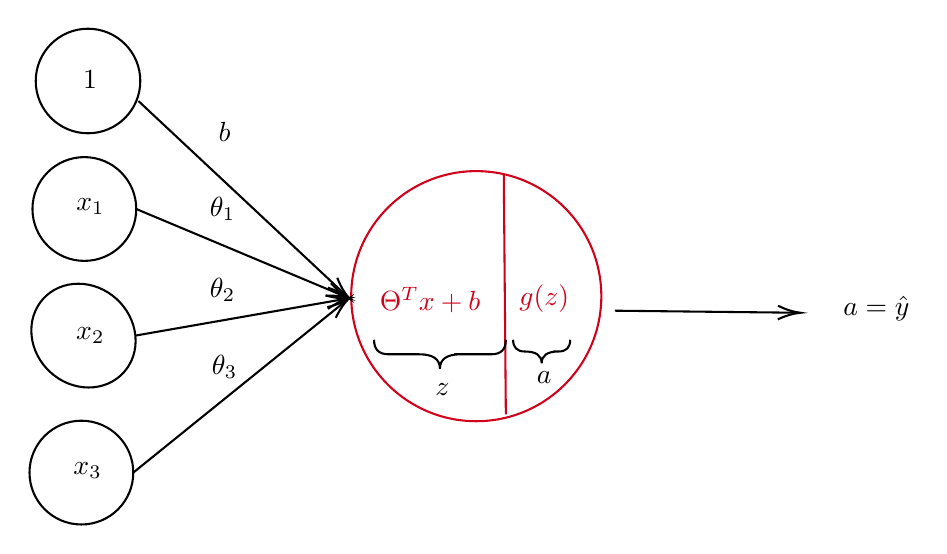
\begin{tikzpicture}[x=0.75pt,y=0.75pt,yscale=-1,xscale=1]
%uncomment if require: \path (0,300); %set diagram left start at 0, and has height of 300

%Shape: Circle [id:dp4894456216466021] 
\draw   (73.43,102) .. controls (73.43,88.19) and (84.63,77) .. (98.43,77) .. controls (112.24,77) and (123.43,88.19) .. (123.43,102) .. controls (123.43,115.81) and (112.24,127) .. (98.43,127) .. controls (84.63,127) and (73.43,115.81) .. (73.43,102) -- cycle ;
%Shape: Circle [id:dp5135503842228779] 
\draw   (73,163) .. controls (71.62,149.19) and (81.69,138) .. (95.5,138) .. controls (109.31,138) and (121.62,149.19) .. (123,163) .. controls (124.38,176.81) and (114.31,188) .. (100.5,188) .. controls (86.69,188) and (74.38,176.81) .. (73,163) -- cycle ;
%Shape: Circle [id:dp5054751399658592] 
\draw   (72,229) .. controls (72,215.19) and (83.19,204) .. (97,204) .. controls (110.81,204) and (122,215.19) .. (122,229) .. controls (122,242.81) and (110.81,254) .. (97,254) .. controls (83.19,254) and (72,242.81) .. (72,229) -- cycle ;
%Shape: Circle [id:dp7068247835752886] 
\draw  [color={rgb, 255:red, 208; green, 2; blue, 27 }  ,draw opacity=1 ] (227,144) .. controls (227,110.72) and (253.97,83.75) .. (287.25,83.75) .. controls (320.53,83.75) and (347.5,110.72) .. (347.5,144) .. controls (347.5,177.28) and (320.53,204.25) .. (287.25,204.25) .. controls (253.97,204.25) and (227,177.28) .. (227,144) -- cycle ;
%Straight Lines [id:da3951259360286594] 
\draw    (123.43,102) -- (224.16,144.23) ;
\draw [shift={(226,145)}, rotate = 202.75] [color={rgb, 255:red, 0; green, 0; blue, 0 }  ][line width=0.75]    (10.93,-3.29) .. controls (6.95,-1.4) and (3.31,-0.3) .. (0,0) .. controls (3.31,0.3) and (6.95,1.4) .. (10.93,3.29)   ;

%Straight Lines [id:da17712089576257095] 
\draw    (123,163) -- (224.03,145.34) ;
\draw [shift={(226,145)}, rotate = 530.0899999999999] [color={rgb, 255:red, 0; green, 0; blue, 0 }  ][line width=0.75]    (10.93,-3.29) .. controls (6.95,-1.4) and (3.31,-0.3) .. (0,0) .. controls (3.31,0.3) and (6.95,1.4) .. (10.93,3.29)   ;

%Straight Lines [id:da10379609280096158] 
\draw    (122,229) -- (224.44,146.26) ;
\draw [shift={(226,145)}, rotate = 501.07] [color={rgb, 255:red, 0; green, 0; blue, 0 }  ][line width=0.75]    (10.93,-3.29) .. controls (6.95,-1.4) and (3.31,-0.3) .. (0,0) .. controls (3.31,0.3) and (6.95,1.4) .. (10.93,3.29)   ;

%Straight Lines [id:da1555895906794451] 
\draw    (354,151) -- (441.5,151.98) ;
\draw [shift={(443.5,152)}, rotate = 180.64] [color={rgb, 255:red, 0; green, 0; blue, 0 }  ][line width=0.75]    (10.93,-3.29) .. controls (6.95,-1.4) and (3.31,-0.3) .. (0,0) .. controls (3.31,0.3) and (6.95,1.4) .. (10.93,3.29)   ;

%Shape: Circle [id:dp07492513539205437] 
\draw   (75,40.33) .. controls (75,26.42) and (86.28,15.14) .. (100.19,15.14) .. controls (114.1,15.14) and (125.38,26.42) .. (125.38,40.33) .. controls (125.38,54.24) and (114.1,65.52) .. (100.19,65.52) .. controls (86.28,65.52) and (75,54.24) .. (75,40.33) -- cycle ;
%Straight Lines [id:da37710728737628485] 
\draw    (124.5,50) -- (224.54,143.63) ;
\draw [shift={(226,145)}, rotate = 223.11] [color={rgb, 255:red, 0; green, 0; blue, 0 }  ][line width=0.75]    (10.93,-3.29) .. controls (6.95,-1.4) and (3.31,-0.3) .. (0,0) .. controls (3.31,0.3) and (6.95,1.4) .. (10.93,3.29)   ;

%Straight Lines [id:da9942335357246543] 
\draw [color={rgb, 255:red, 208; green, 2; blue, 27 }  ,draw opacity=1 ]   (300.5,85) -- (301.5,201) ;


%Shape: Brace [id:dp48208896309529936] 
\draw   (238,165) .. controls (238,169.67) and (240.33,172) .. (245,172) -- (259.75,172) .. controls (266.42,172) and (269.75,174.33) .. (269.75,179) .. controls (269.75,174.33) and (273.08,172) .. (279.75,172)(276.75,172) -- (294.5,172) .. controls (299.17,172) and (301.5,169.67) .. (301.5,165) ;
%Shape: Brace [id:dp308784031815875] 
\draw   (305,165) .. controls (305,168.77) and (306.89,170.66) .. (310.66,170.66) -- (310.66,170.66) .. controls (316.05,170.66) and (318.75,172.55) .. (318.75,176.32) .. controls (318.75,172.55) and (321.45,170.66) .. (326.84,170.66)(324.41,170.66) -- (326.84,170.66) .. controls (330.61,170.66) and (332.5,168.77) .. (332.5,165) ;

% Text Node
\draw (101.3,163) node   {$x_{2}$};
% Text Node
\draw (101.37,100.96) node   {$x_{1}$};
% Text Node
\draw (100,228) node   {$x_{3}$};
% Text Node
\draw (101.21,39.84) node   {$1$};
% Text Node
\draw (166,65) node   {$b$};
% Text Node
\draw (165,102) node   {$\theta _{1}$};
% Text Node
\draw (165,141) node   {$\theta _{2}$};
% Text Node
\draw (166,178) node   {$\theta _{3}$};
% Text Node
\draw (480,150) node   {$a=\hat{y}$};
% Text Node
\draw (320,145) node [color={rgb, 255:red, 208; green, 2; blue, 27 }  ,opacity=1 ]  {$g( z)$};
% Text Node
\draw (265,146) node [color={rgb, 255:red, 208; green, 2; blue, 27 }  ,opacity=1 ]  {$\Theta ^{T} x+b$};
% Text Node
\draw (271,189) node   {$z$};
% Text Node
\draw (320,183) node   {$a$};


\end{tikzpicture}


}
\caption{Single layer neural network. The input $x$ is multiplied by the matrix of weights $\Theta$ to be passed to the activation function (a typically non-linear function to transform the input) to generate the output $\hat { y }$. \protect \footnotemark}
% BR: you should also mention the activation function here and give an
% example.
\label{fig:preceptron}
\end{figure}
\footnotetext{The figure is adapted from https://www.coursera.org/learn/machine-learning.}
\noindent
Despite neural networks being the new trend in machine learning, they are rather old algorithms, which are motivated by the goal of having a machine that mimics a brain. The sudden resurgence of neural networks is due to the fact that they are computationally expensive and require a huge amounts of data, which was neither available nor processable in the 80s and 90s. Also \emph{``backpropagation''} algorithm~\brackettext{\cite{SCHOL:journals/nature/rumelhart1986learning}} and the advent of GPUs, sped up the training process and made it feasible to train models with thousands of parameters.\\
A single artificial neuron, consisting of a single computational unit, is shown in Figure~\ref{fig:preceptron}. The computational unit illustrated in red takes in the different features of the input $x_i$ and multiplies each with a given weight $\theta_i$. The result of the multiplication is added to the \emph{bias unit} $b$ that always has an input value of $1$.
The weights indicate the importance of each feature for the computation and are learnable parameters of the model. The neuron then performs a transformation to the input through the \emph{activation function} ($g(x)$) and generates the output ($\hat { y } $). The activation function is typically non-linear transformation that is applied on the input data.\\
% BR: the non-linearity arises from the activation function; you should
% mention this. Moreover, you can select a linear activation function if
% you want.  I would thus rather say that they are 'typically selected
% to be non-linear' or something similar.
Essentially, each neuron consists of two steps of computation. First, intermediate output $z$ is computed by the multiplication of weights with input features, which is a linear operation that boils down to a matrix--vector product.
Second, an activation function of choice is applied to $z$ to produce the final output or activation ($a$) of the last unit. \\
\begin{figure}
\centering 
\resizebox{0.75\textwidth}{0.45\textwidth}{      
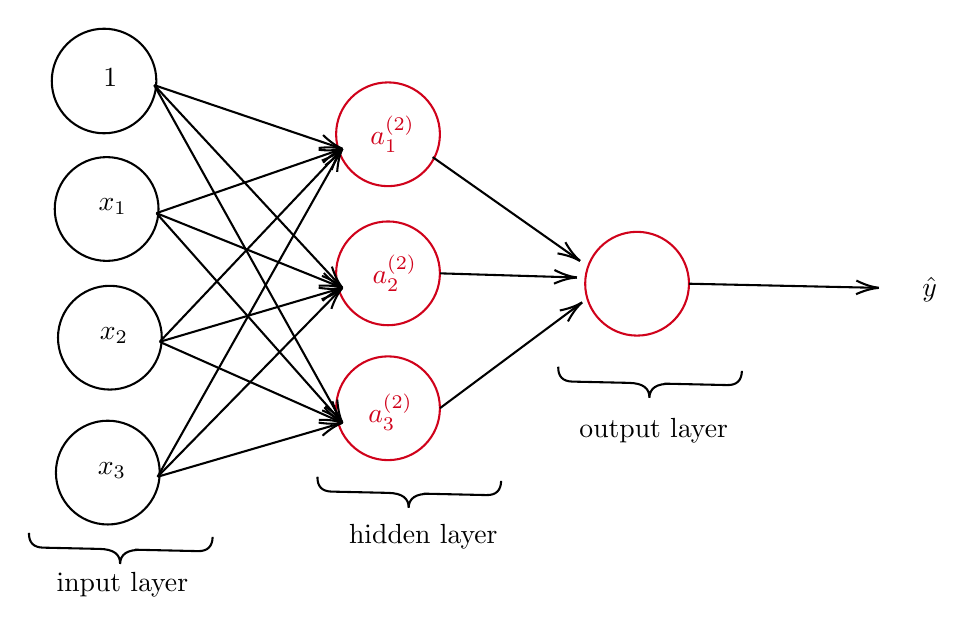
\begin{tikzpicture}[x=0.75pt,y=0.75pt,yscale=-1,xscale=1]
%uncomment if require: \path (0,300); %set diagram left start at 0, and has height of 300

\draw  [color={rgb, 255:red, 208; green, 2; blue, 27 }  ,draw opacity=1 ]  (241, 71) circle [x radius= 25, y radius= 25]  ;
\draw  [color={rgb, 255:red, 208; green, 2; blue, 27 }  ,draw opacity=1 ]  (241, 138) circle [x radius= 25, y radius= 25]  ;
\draw  [color={rgb, 255:red, 208; green, 2; blue, 27 }  ,draw opacity=1 ]  (241, 203) circle [x radius= 25, y radius= 25]  ;
\draw    (262.5,82) -- (333.5,132) ;
\draw [shift={(333.5,132)}, rotate = 215.15] [color={rgb, 255:red, 0; green, 0; blue, 0 }  ]   (0,0) .. controls (3.31,-0.3) and (6.95,-1.4) .. (10.93,-3.29)(0,0) .. controls (3.31,0.3) and (6.95,1.4) .. (10.93,3.29)   ;

\draw    (266,138) -- (332,140) ;
\draw [shift={(332,140)}, rotate = 181.74] [color={rgb, 255:red, 0; green, 0; blue, 0 }  ]   (0,0) .. controls (3.31,-0.3) and (6.95,-1.4) .. (10.93,-3.29)(0,0) .. controls (3.31,0.3) and (6.95,1.4) .. (10.93,3.29)   ;

\draw    (266,203) -- (334.5,152) ;
\draw [shift={(334.5,152)}, rotate = 503.33] [color={rgb, 255:red, 0; green, 0; blue, 0 }  ]   (0,0) .. controls (3.31,-0.3) and (6.95,-1.4) .. (10.93,-3.29)(0,0) .. controls (3.31,0.3) and (6.95,1.4) .. (10.93,3.29)   ;

\draw  [color={rgb, 255:red, 208; green, 2; blue, 27 }  ,draw opacity=1 ]  (361, 143) circle [x radius= 25, y radius= 25]  ;
\draw    (386,143) -- (477.5,145) ;
\draw [shift={(477.5,145)}, rotate = 181.25] [color={rgb, 255:red, 0; green, 0; blue, 0 }  ]   (0,0) .. controls (3.31,-0.3) and (6.95,-1.4) .. (10.93,-3.29)(0,0) .. controls (3.31,0.3) and (6.95,1.4) .. (10.93,3.29)   ;

\draw    (105.43, 107) circle [x radius= 25, y radius= 25]  ;
\draw    (107, 169) circle [x radius= 25, y radius= 25]  ;
\draw    (106, 234) circle [x radius= 25, y radius= 25]  ;
\draw    (104.19, 45.33) circle [x radius= 25.19, y radius= 25.19]  ;
\draw    (128.38,47.33) -- (219,78) ;
\draw [shift={(219,78)}, rotate = 198.7] [color={rgb, 255:red, 0; green, 0; blue, 0 }  ]   (0,0) .. controls (3.31,-0.3) and (6.95,-1.4) .. (10.93,-3.29)(0,0) .. controls (3.31,0.3) and (6.95,1.4) .. (10.93,3.29)   ;

\draw    (128.38,47.33) -- (219,145) ;
\draw [shift={(219,145)}, rotate = 227.14] [color={rgb, 255:red, 0; green, 0; blue, 0 }  ]   (0,0) .. controls (3.31,-0.3) and (6.95,-1.4) .. (10.93,-3.29)(0,0) .. controls (3.31,0.3) and (6.95,1.4) .. (10.93,3.29)   ;

\draw    (128.38,47.33) -- (219,210) ;
\draw [shift={(219,210)}, rotate = 240.88] [color={rgb, 255:red, 0; green, 0; blue, 0 }  ]   (0,0) .. controls (3.31,-0.3) and (6.95,-1.4) .. (10.93,-3.29)(0,0) .. controls (3.31,0.3) and (6.95,1.4) .. (10.93,3.29)   ;

\draw    (129.43,109) -- (219,210) ;
\draw [shift={(219,210)}, rotate = 228.43] [color={rgb, 255:red, 0; green, 0; blue, 0 }  ]   (0,0) .. controls (3.31,-0.3) and (6.95,-1.4) .. (10.93,-3.29)(0,0) .. controls (3.31,0.3) and (6.95,1.4) .. (10.93,3.29)   ;

\draw    (129.43,109) -- (219,145) ;
\draw [shift={(219,145)}, rotate = 201.9] [color={rgb, 255:red, 0; green, 0; blue, 0 }  ]   (0,0) .. controls (3.31,-0.3) and (6.95,-1.4) .. (10.93,-3.29)(0,0) .. controls (3.31,0.3) and (6.95,1.4) .. (10.93,3.29)   ;

\draw    (129.43,109) -- (219,78) ;
\draw [shift={(219,78)}, rotate = 520.9100000000001] [color={rgb, 255:red, 0; green, 0; blue, 0 }  ]   (0,0) .. controls (3.31,-0.3) and (6.95,-1.4) .. (10.93,-3.29)(0,0) .. controls (3.31,0.3) and (6.95,1.4) .. (10.93,3.29)   ;

\draw    (131,171) -- (219,78) ;
\draw [shift={(219,78)}, rotate = 493.42] [color={rgb, 255:red, 0; green, 0; blue, 0 }  ]   (0,0) .. controls (3.31,-0.3) and (6.95,-1.4) .. (10.93,-3.29)(0,0) .. controls (3.31,0.3) and (6.95,1.4) .. (10.93,3.29)   ;

\draw    (131,171) -- (219,145) ;
\draw [shift={(219,145)}, rotate = 523.54] [color={rgb, 255:red, 0; green, 0; blue, 0 }  ]   (0,0) .. controls (3.31,-0.3) and (6.95,-1.4) .. (10.93,-3.29)(0,0) .. controls (3.31,0.3) and (6.95,1.4) .. (10.93,3.29)   ;

\draw    (131,171) -- (219,210) ;
\draw [shift={(219,210)}, rotate = 203.9] [color={rgb, 255:red, 0; green, 0; blue, 0 }  ]   (0,0) .. controls (3.31,-0.3) and (6.95,-1.4) .. (10.93,-3.29)(0,0) .. controls (3.31,0.3) and (6.95,1.4) .. (10.93,3.29)   ;

\draw    (130,236) -- (219,78) ;
\draw [shift={(219,78)}, rotate = 479.39] [color={rgb, 255:red, 0; green, 0; blue, 0 }  ]   (0,0) .. controls (3.31,-0.3) and (6.95,-1.4) .. (10.93,-3.29)(0,0) .. controls (3.31,0.3) and (6.95,1.4) .. (10.93,3.29)   ;

\draw    (130,236) -- (219,145) ;
\draw [shift={(219,145)}, rotate = 494.36] [color={rgb, 255:red, 0; green, 0; blue, 0 }  ]   (0,0) .. controls (3.31,-0.3) and (6.95,-1.4) .. (10.93,-3.29)(0,0) .. controls (3.31,0.3) and (6.95,1.4) .. (10.93,3.29)   ;

\draw    (130,236) -- (219,210) ;
\draw [shift={(219,210)}, rotate = 523.72] [color={rgb, 255:red, 0; green, 0; blue, 0 }  ]   (0,0) .. controls (3.31,-0.3) and (6.95,-1.4) .. (10.93,-3.29)(0,0) .. controls (3.31,0.3) and (6.95,1.4) .. (10.93,3.29)   ;

\draw   (68,263) .. controls (67.89,267.67) and (70.17,270.05) .. (74.84,270.16) -- (102.1,270.77) .. controls (108.76,270.92) and (112.04,273.32) .. (111.93,277.99) .. controls (112.04,273.32) and (115.42,271.07) .. (122.09,271.22)(119.09,271.15) -- (149.34,271.83) .. controls (154.01,271.94) and (156.39,269.66) .. (156.5,264.99) ;
\draw   (207,236) .. controls (206.89,240.67) and (209.17,243.05) .. (213.84,243.16) -- (241.1,243.77) .. controls (247.76,243.92) and (251.04,246.32) .. (250.93,250.99) .. controls (251.04,246.32) and (254.42,244.07) .. (261.09,244.22)(258.09,244.15) -- (288.34,244.83) .. controls (293.01,244.94) and (295.39,242.66) .. (295.5,237.99) ;
\draw   (323,183) .. controls (322.89,187.67) and (325.17,190.05) .. (329.84,190.16) -- (357.1,190.77) .. controls (363.76,190.92) and (367.04,193.32) .. (366.93,197.99) .. controls (367.04,193.32) and (370.42,191.07) .. (377.09,191.22)(374.09,191.15) -- (404.34,191.83) .. controls (409.01,191.94) and (411.39,189.66) .. (411.5,184.99) ;

\draw (243.21,70.84) node [color={rgb, 255:red, 208; green, 2; blue, 27 }  ,opacity=1 ]  {$a^{( 2)}_{1}$};
\draw (244.21,137.84) node [color={rgb, 255:red, 208; green, 2; blue, 27 }  ,opacity=1 ]  {$a^{( 2)}_{2}$};
\draw (242.21,204.84) node [color={rgb, 255:red, 208; green, 2; blue, 27 }  ,opacity=1 ]  {$a^{( 2)}_{3}$};
\draw (109,168) node   {$x_{2}$};
\draw (108.37,105.96) node   {$x_{1}$};
\draw (108,233) node   {$x_{3}$};
\draw (107.21,43.84) node   {$1$};
\draw (502,146) node   {$\hat{y}$};
\draw (113,288) node   {input layer};
\draw (258,265) node   {hidden layer};
\draw (369,214) node   {output layer};


\end{tikzpicture}

}
\caption{Two layer neural network with one hidden layer. An input $x$ with three features is multiplied by the weight matrix $\Theta$ to generate an intermediate activation value $a$. The predicted output $\hat { y } $ is generated using the activations of the hidden layer.  \protect \footnotemark .}

\label{fig:nn}

\end{figure}
\noindent
A neural network is a group of multiple neurons connected together, as shown in Figure~\ref{fig:nn}. In a neural network, the first layer is called the \emph{input layer}, the last layer is called the \emph{output layer} and all other layers are referred to as \emph{hidden layers}.
Typically, the values of the input and the output layer (labels) are given in the training set. The output of each computational unit in the network is the activation of that unit. We denote activation of the unit (neuron) $i$ in layer $j$ by $a_{i}^{[j]}$. The weights of the network are the parameters of the model and learning them is goal of any neural network. We denote the weight controlling the function mapping from unit $n$ in layer $j$ to unit $l$ in layer $j+1$ by
$\theta^{(j)}_{nl}$. The weights indicate how different features of inputs should be combined and how much should each of them influence the final output. The values of intermediate activations can be interpreted as latent features discovered during training~\brackettext{\cite{SCHOL:book/haykin2009}}. As the network gets deeper, more complex combinations of input features can be learned. \\
An example of forward computation, which is called \emph{forward propagation}, for the network in Figure~\ref{fig:nn} is given in Equation~\ref{eq:nn_eq}. Although a single output is shown the figure, the output layer can have different sizes. It can vary from one output for a single class classification even $10,000$ pixels of a image. The number of hidden layers can also vary, where the next hidden layer would use the activation of the pervious layer as input. How different neurons connect, the choice of activation function, the shape of the output layer and the number of layers is what defines different architectures~\brackettext{\cite{SCHOL:Goodfellow-et-al-2016}}. Since most of literature on word embeddings focus on shallow neural networks, in this thesis, we focus only on networks with a few hidden layers. 
\begin{equation}
\begin{split}
a_{ 1 }^{ [2] }=g(\theta _{ 10 }^{ [1] }x_{ 0 }+\theta _{ 11 }^{ [1]}x_{ 1 }+\theta _{ 12 }^{ [1] }x_{ 2 }+\theta _{ 13 }^{ [1] }x_{ 3 })\\ 
a_{ 2 }^{ [2] }=g(\theta _{ 20 }^{ [1] }x_{ 0 }+\theta _{ 21 }^{ [1] }x_{ 1 }+\theta _{ 22 }^{ [1] }x_{ 2 }+\theta _{ 23 }^{ [1] }x_{ 3 })\\
 a_{ 3 }^{ [2] }=g(\theta _{ 30 }^{ [1] }x_{ 0 }+\theta _{ 31 }^{ [1] }x_{ 1 }+\theta _{ 32 }^{ [1] }x_{ 2 }+\theta _{ 33 }^{ [1] }x_{ 3 })\\
  \hat { y } =a_{ 1 }^{ [3] }=g(\theta _{ 10 }^{ [2] }x_{ 0 }+\theta _{ 11 }^{ [2] }x_{ 1 }+\theta _{ 12 }^{ [2] }x_{ 2 }+\theta _{ 13 }^{ [2] }x_{ 3 })
\end{split}
\label{eq:nn_eq}
\end{equation}
\footnotetext{The figure is adapted from https://www.coursera.org/learn/neural-networks-deep-learning.}
Activation functions are an important part of neural networks, without them the networks are just weighted sum of their inputs, plus a bias term that are unable to learn any complex and non-linear function. Activation functions are means to introduce non-linearity to the model. There are different classes of activation functions available but the most commonly used ones are \emph{Sigmoid} and \emph{Relu}, both them are illustrated in Figure~\ref{fig:activation}. 
% BR: This is a good introduction to DL. At times, the 'flow' of the
% section is not optimal, though. This is partially caused by terms,
% i.e. concepts, that are mentioned but not explained. It is perfect
% to just briefly explain a term once before using it.
%TODO : when you read again take this comment into account 
% Example: 'Calculating the output of a neural network based on
% a certain input vector $x$ is commonly referred to as \emph{forward
% computation}. Equation X shows an example of a forward computation
% of the network shown in Figure Y.

\begin{figure}
\centering
\subcaptionbox{\label{sfig:relu}}{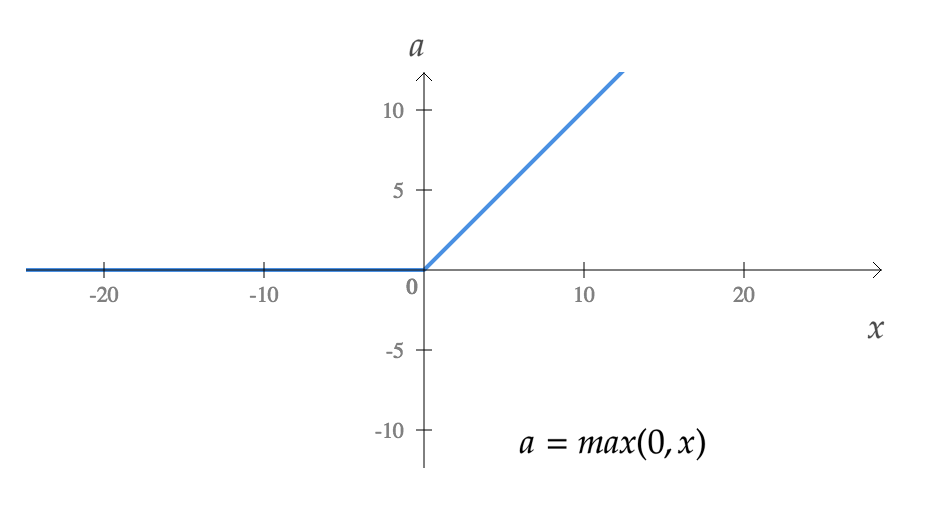
\includegraphics[width=0.45\linewidth , height=0.33\linewidth]{images/relu.png}}
\subcaptionbox{\label{sfig:sigmoid}}{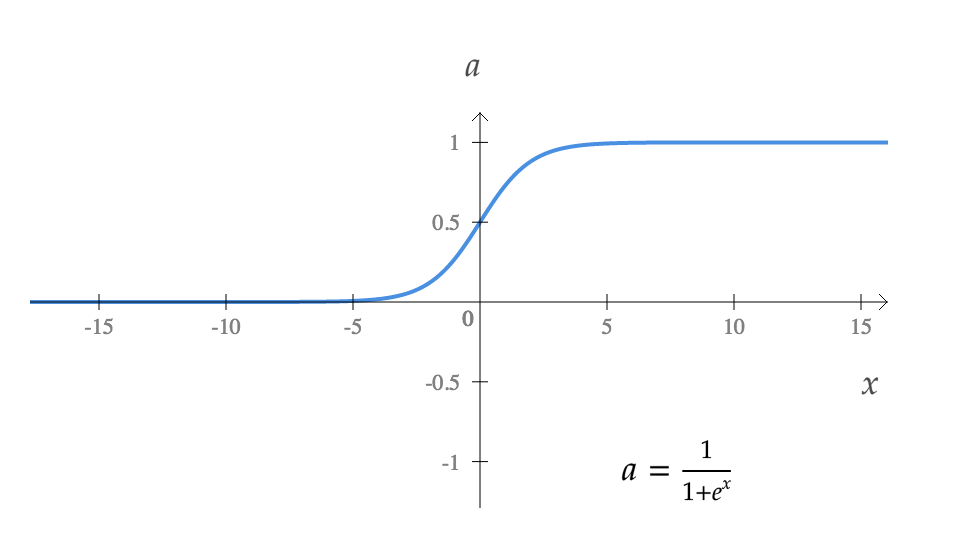
\includegraphics[width=0.45\linewidth , height=0.33\linewidth]{images/sigmoid.png}}
\caption{Common choices of activation functions are ~\subref{sfig:relu} Relu function $a=\mathrm{max}(0,x)$, which cuts values below zero and ~\subref{sfig:sigmoid} Sigmoid function $a=\frac{1}{1+e^{x}}$, which forces the values to be between zero and one.}
\label{fig:activation}
\end{figure}
%%%%%%%%%%%%%%%%%%%%%%%%%%%%%%%%%%%%%%%%%%%%%%%%%%%%%%%%%%%%
\subsection{Training neural networks}
Consider the output $\hat { y } $ as the prediction of our network for some task. In a supervised learning problem, the aim is to reduce the error between the prediction ($\hat { y } $) and the true label $y$. As a result, a cost function on parameters $\theta$ and $b$ is defined as $J$ in Equation~\ref{eq:cost_nn}, where $L$ denotes the loss function on a single training example and $m$ is the size of the training set. The \emph{cost function} is simply the sum of all losses on the training set.
% BR: you should briefly mention what types of loss functions exist, or
% use a simple one (MSE or something?)
\begin{equation}
J(\theta,b)=\sum _{ j=1 }^{ m }{ L( } \hat { y }^{ (i) } ,y^{ (i) })
\label{eq:cost_nn}
\end{equation}
The loss for a single input is computed by the \emph{loss function} $L$ and the sum of loses for all inputs is computed by the cost function $J$. There exists various loss functions, which are chosen based on the problem at hand. We introduce three of the most commonly used loss functions, which are used by the models in this thesis: \\
\begin{inparaenum}
\item \emph{Mean Squared Error} (MSE) or \emph{quadratic cost} minimizes the quadratic sum of distances between true label of each data point $y^{ (i) }$ and it's prediction $\hat { y } ^{ (i) }$~\brackettext{\cite{DBLP:reference/ml/2017}}: 
\begin{equation}
L=\frac { 1 }{ n } \sum _{ i=1 }^{ n }{ (\hat { y } ^{ (i) }- } y^{ (i) })^{ 2 }
\end{equation}
\item \emph{Kullback Leibler (KL) Divergence} also known as relative entropy, is a measure of how one probability distribution $y^{ (i) }$ (predicted distribution) diverges from a second probability distribution $\hat { y } ^{ (i) }$ (true distribution), the higher is the KL divergence, the more different the are distributions. KL divergence is not symmetric: The KL from $y^{ (i) }$ to $\hat { y } ^{ (i) }$ is generally not the same as the KL from $\hat { y } ^{ (i) }$ to $y^{ (i) }$~\brackettext{\cite{DBLP:books/daglib/0016881}}. The formula consists of two parts, where the first part is called \emph{entropy} and the second part \emph{cross-entropy}.
\begin{equation}
\begin{split}
L=\frac { 1 }{ n } \sum _{ i=1 }^{ n }{ D_{ kl }(y^{ (i) }||\hat { y } ^{ (i) }) } =\\
 \frac { 1 }{ n } \sum _{ i=1 }^{ n }{ (y^{ (i) }\log{(\frac { y^{ (i) } }{ \hat { y } ^{ (i) } } )) }} =\\
 \underbrace { \frac { 1 }{ n } \sum _{ i=1 }^{ n }{ (y^{ (i) }\log{(y^{ (i) })) }} - }_{ entropy } \underbrace { \frac { 1 }{ n } \sum _{ i=1 }^{ n }{ (y^{ (i) }\log{(\hat { y } ^{ (i) })) }}  }_{ cross-entropy } 
 \end{split}
\end{equation}
\item \emph{Cross Entropy} is commonly-used where labels are assumed to take only two values and corresponds to the second part of KL divergence formula, where the second distribution $\hat { y } ^{ (i) }$ is fixed~\brackettext{\cite{DBLP:books/daglib/0016881}}. The cross entropy for a classification problem with two classes is defined as:  
\begin{equation}
L=-\frac { 1 }{ n } \sum _{ i=1 }^{ n }{ [y^{ (i) }\log{(\hat { y } ^{ (i) })+(1-  y^{ (i) }}})\log{(1-\hat { y } ^{ (i) }})
\end{equation}
\end{inparaenum}
The goal of the training phase is to learn a weight matrix $\Theta$ and a bias term $b$ such that the overall cost is minimized. This naturally leads to an optimisation problem, which is  typically solved using \emph{Gradient Descent} (GD)~\brackettext{\cite{DBLP:journals/corr/Ruder16}}.
Gradient descent is a way to minimize an objective function by finding local minima based on local gradients.
% BR: I slightly object to that description. I would drop the
% 'parameterized ...' part and just leave it as 'a way to minimize an
% objective function by finding local minima based on local gradients'
% or something like that.
It is an iterative algorithm, where in each step parameters of the model are updated using the gradient of the function. A single step of GD  for one parameter $\theta$ can be seen in Equation~\ref{eq:gd}, where the previous value of the parameter is updated based on the gradient of the cost function in respect with $\theta$. Here, $\alpha$ is the \emph{learning rate} or the step size and controls the magnitude of the update in each iteration. 
\begin{equation}
\theta=: \theta- \alpha\frac { \partial J(\theta) }{ \partial \theta }
\label{eq:gd}
\end{equation}
In a dataset with $m$ training examples, for each training example, the gradient of the cost function with respect to every weight and bias has to be calculated and accumulated.
After iterating through all the training examples the weights and bias terms will be updated by the accumulate sum. This process is repeated for some number of iterations, where each iteration is one pass through the training set. Because the number of training examples for deep learning models are usually large, variations of GD have been introduce to speed up the process, three main type of GD are as follows: 
\begin{itemize}
\item \textbf{Mini-batch GD:} Instead of iterating over all training examples, a subset of a batch, i.e.,\ a subset of the input data, is considered, before making an update, making it a good choice very large datasets.
\item \textbf{Stochastic-GD:} In this case, only one example is looked at, before making an update. 
\item \textbf{Batch-GD:} The original algorithm with iteration over all examples. 
% BR: It's inconsistent to refer to it as a variation of the algorithm,
% though, right?
\end{itemize} 
Considering the most simple case (a function with only one parameter) gradient descent is illustrated in Figure~\ref{fig:gradientD}. As shown in the figure, the derivative or the slope of the function is positive on the right side of the minimum (the update rule will decrease $\theta$) and negative on the left size (the update rule will increase $\theta$). The same rule holds in higher dimensions as well. Although the figure illustrates a function with global minimum, it is worth noting that GD is not guaranteed to find the global minimum and is often stuck in local minima.\\
% BR: This is very nice. To be mathematically airtight, you could write
% that this holds in higher dimensions as well. However, one may require
% approximations of the gradient there, of course.
%
%\begin{algorithm}[htbp]
%  %
%  \begin{algorithmic}[1]
%    \newcommand{\UF}{\mathrm{U}}
%   \While{(not converged)}
% \State $\theta=: \theta- \alpha\frac { \partial J(\theta) }{ \partial \theta } $
%  \EndWhile
%  \end{algorithmic}
%  %
%\caption{: Gradient decent}
% \label{algo:gd}
%\end{algorithm}

\begin{figure}
\centering 
\resizebox{0.65\textwidth}{0.4\textwidth}{      
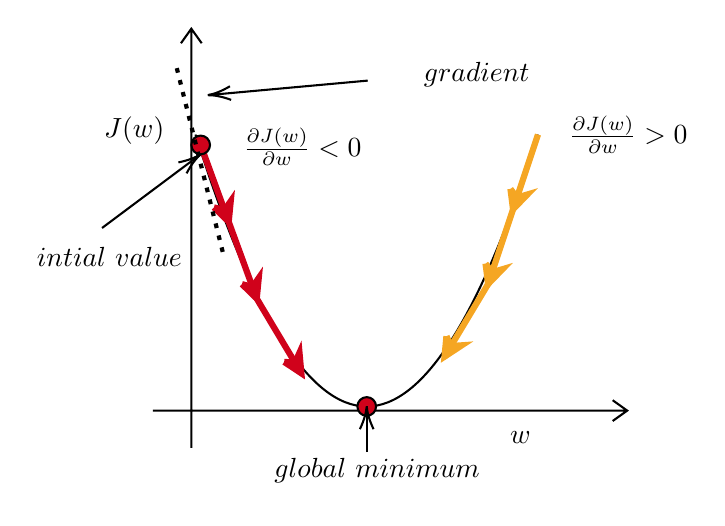
\begin{tikzpicture}[x=0.75pt,y=0.75pt,yscale=-1,xscale=1]
%uncomment if require: \path (0,300); %set diagram left start at 0, and has height of 300

\draw  (75,190) -- (303.5,190)(93.5,6) -- (93.5,208) (296.5,185) -- (303.5,190) -- (296.5,195) (88.5,13) -- (93.5,6) -- (98.5,13)  ;
\draw   (95.5,57) .. controls (150.5,231.67) and (205.5,231.67) .. (260.5,57) ;
\draw [color={rgb, 255:red, 208; green, 2; blue, 27 }  ,draw opacity=1 ][line width=2.25]    (98,62) -- (111.5,99) ;
\draw [shift={(111.5,99)}, rotate = 249.95] [color={rgb, 255:red, 208; green, 2; blue, 27 }  ,draw opacity=1 ][fill={rgb, 255:red, 208; green, 2; blue, 27 }  ,fill opacity=1 ][line width=2.25]   (8.93,-4.29) -- (0,0) -- (8.93,4.29) -- (5.93,0) -- (8.93,-4.29)    ;

\draw [color={rgb, 255:red, 208; green, 2; blue, 27 }  ,draw opacity=1 ][line width=2.25]    (111.5,99) -- (125,136) ;
\draw [shift={(125,136)}, rotate = 249.95] [color={rgb, 255:red, 208; green, 2; blue, 27 }  ,draw opacity=1 ][fill={rgb, 255:red, 208; green, 2; blue, 27 }  ,fill opacity=1 ][line width=2.25]   (8.93,-4.29) -- (0,0) -- (8.93,4.29) -- (5.93,0) -- (8.93,-4.29)    ;

\draw [color={rgb, 255:red, 208; green, 2; blue, 27 }  ,draw opacity=1 ][line width=2.25]    (125,136) -- (146.5,172) ;
\draw [shift={(146.5,172)}, rotate = 239.15] [color={rgb, 255:red, 208; green, 2; blue, 27 }  ,draw opacity=1 ][fill={rgb, 255:red, 208; green, 2; blue, 27 }  ,fill opacity=1 ][line width=2.25]   (8.93,-4.29) -- (0,0) -- (8.93,4.29) -- (5.93,0) -- (8.93,-4.29)    ;

\draw [color={rgb, 255:red, 245; green, 166; blue, 35 }  ,draw opacity=1 ][line width=2.25]    (260.5,57) -- (248.5,93) ;
\draw [shift={(248.5,93)}, rotate = 288.43] [color={rgb, 255:red, 245; green, 166; blue, 35 }  ,draw opacity=1 ][fill={rgb, 255:red, 245; green, 166; blue, 35 }  ,fill opacity=1 ][line width=2.25]   (8.93,-4.29) -- (0,0) -- (8.93,4.29) -- (5.93,0) -- (8.93,-4.29)    ;

\draw [color={rgb, 255:red, 245; green, 166; blue, 35 }  ,draw opacity=1 ][line width=2.25]    (248.5,93) -- (236.5,129) ;
\draw [shift={(236.5,129)}, rotate = 288.43] [color={rgb, 255:red, 245; green, 166; blue, 35 }  ,draw opacity=1 ][fill={rgb, 255:red, 245; green, 166; blue, 35 }  ,fill opacity=1 ][line width=2.25]   (8.93,-4.29) -- (0,0) -- (8.93,4.29) -- (5.93,0) -- (8.93,-4.29)    ;

\draw [color={rgb, 255:red, 245; green, 166; blue, 35 }  ,draw opacity=1 ][line width=2.25]    (236.5,129) -- (215.5,164) ;
\draw [shift={(215.5,164)}, rotate = 300.96] [color={rgb, 255:red, 245; green, 166; blue, 35 }  ,draw opacity=1 ][fill={rgb, 255:red, 245; green, 166; blue, 35 }  ,fill opacity=1 ][line width=2.25]   (8.93,-4.29) -- (0,0) -- (8.93,4.29) -- (5.93,0) -- (8.93,-4.29)    ;

\draw  [fill={rgb, 255:red, 208; green, 2; blue, 27 }  ,fill opacity=1 ]  (98, 62) circle [x radius= 4.5, y radius= 4.5]  ;
\draw    (50.5,102) -- (98,66.5) ;
\draw [shift={(98,66.5)}, rotate = 503.23] [color={rgb, 255:red, 0; green, 0; blue, 0 }  ]   (0,0) .. controls (3.31,-0.3) and (6.95,-1.4) .. (10.93,-3.29)(0,0) .. controls (3.31,0.3) and (6.95,1.4) .. (10.93,3.29)   ;

\draw  [fill={rgb, 255:red, 208; green, 2; blue, 27 }  ,fill opacity=1 ]  (178, 188) circle [x radius= 4.5, y radius= 4.5]  ;
\draw    (178,210) -- (178,188) ;
\draw [shift={(178,188)}, rotate = 450] [color={rgb, 255:red, 0; green, 0; blue, 0 }  ]   (0,0) .. controls (3.31,-0.3) and (6.95,-1.4) .. (10.93,-3.29)(0,0) .. controls (3.31,0.3) and (6.95,1.4) .. (10.93,3.29)   ;

\draw [line width=1.5]  [dash pattern={on 1.69pt off 2.76pt}]  (86.5,25) -- (109.5,117) ;


\draw    (178.5,31) -- (101.5,38) ;
\draw [shift={(101.5,38)}, rotate = 354.81] [color={rgb, 255:red, 0; green, 0; blue, 0 }  ]   (0,0) .. controls (3.31,-0.3) and (6.95,-1.4) .. (10.93,-3.29)(0,0) .. controls (3.31,0.3) and (6.95,1.4) .. (10.93,3.29)   ;


\draw (252,203) node   {$w$};
\draw (66,55) node   {$J( w)$};
\draw (147,63) node   {$\frac{\partial J( w)}{\partial w} < 0$};
\draw (304,57) node   {$\frac{\partial J( w)}{\partial w}  >0$};
\draw (183,219) node   {$global\ minimum$};
\draw (54,116) node   {$intial\ value$};
\draw (231,28) node   {$gradient$};


\end{tikzpicture}

}
\caption{Gradient decent on a one-dimensional function with only one parameter.
In each iteration, we take a step in the direction of the gradient. The gradient will guide the algorithm to the functions local minimum.
% BR: do you want to mention getting stuck in local optima?
}
\label{fig:gradientD}
\end{figure}
\noindent
%%%%%%%%%%%%%%%%%%%%%%%%%%%%%%%%%%%%%%%%%%%%%%%%%%%%%%%%%%%%
\subsection{Embeddings}\label{subsec:embeddings}
One of the challenges of machine learning is to come up with suitable features for algorithms. These features often have to be task-specific and reflect the needs of the downstream tasks, for example, a task that uses embeddings as input features. \emph{Representation learning} attempts to learn good features and representations automatically~\brackettext{\cite{SCHOL:journals/FDS/ZhongWD16}}. \emph{Principle Component Analysis} (PCA)~\brackettext{\cite{DBLP:journals/corr/Shlens14}} is one example of a traditional method for representation learning from high dimensional data. More recently, neural networks are used to obtain these low-dimensional representations. In a deep learning architecture, the output of each intermediate layer can be viewed as a representation of the original input data. Each unit inn the hidden layer of the network computes a non-linear combination of the inputs that is used by the next layer.  If the dimensions of the hidden layer is smaller than the input layer, a low-dimensional representation of the data is learned in the hidden layer. Based on this principle almost any type of data (e.g., images, sounds and text) can be transformed into embeddings with lower dimensions. In this work, we focus on learning low-dimensional representation for two types of data structures, namely, for words (\emph{word embeddings}) and for graphs (\emph{graph embeddings}). \\
Text is inherently high-dimensional, requiring a specific form of embedding.
% BR: The sentence is a little bit too short and disrupts the flow.
% Maybe: 'However, text is inherently high-dimensional, requiring
% a specific form of embedding'.
In most traditional NLP systems, each word is represented as a one-hot vector of the size of the vocabulary, which is a high-dimensional, highly sparse vector. 
By feeding these high-dimensional representations to a neural network with a smaller hidden layer, a new representation (usually in the order of $100$ dimensions) for each word is learned, which is a more dense vector representation for each word. For this purpose, different models have been proposed, the most famous being word2vec~\brackettext{\cite{DBLP:journals/corr/abs-1301-3781}}, which will be discussed in Section~\ref{sec:wordembeddig} in detail. All the models follow the same principle, which is illustrated in Figure~\ref{fig:emb}, where the one-hot vectors of words in the vocabulary are the input of the network and a low-dimensional hidden layer is responsible for encoding the representation of input words.  The size of the output layer depends on the particular architecture and the cost function. In addition, the network can be composed of multiple layers, but for our purposes, we focus on shallow networks with only one hidden layer. \\
\begin{figure}
\centering 
\resizebox{0.8\textwidth}{0.48\textwidth}{      
\begin{tikzpicture}[x=0.75pt,y=0.75pt,yscale=-1,xscale=1]
%uncomment if require: \path (0,406); %set diagram left start at 0, and has height of 406

\draw  [color={rgb, 255:red, 208; green, 2; blue, 27 }  ,draw opacity=1 ]  (302, 69) circle [x radius= 25, y radius= 25]  ;
\draw  [color={rgb, 255:red, 208; green, 2; blue, 27 }  ,draw opacity=1 ]  (301, 135) circle [x radius= 25, y radius= 25]  ;
\draw  [color={rgb, 255:red, 208; green, 2; blue, 27 }  ,draw opacity=1 ]  (301, 200) circle [x radius= 25, y radius= 25]  ;
\draw    (322.5,79) -- (411.5,133) ;
\draw [shift={(411.5,133)}, rotate = 211.25] [color={rgb, 255:red, 0; green, 0; blue, 0 }  ]   (0,0) .. controls (3.31,-0.3) and (6.95,-1.4) .. (10.93,-3.29)(0,0) .. controls (3.31,0.3) and (6.95,1.4) .. (10.93,3.29)   ;

\draw    (326,135) -- (411.5,133) ;
\draw [shift={(411.5,133)}, rotate = 538.6600000000001] [color={rgb, 255:red, 0; green, 0; blue, 0 }  ]   (0,0) .. controls (3.31,-0.3) and (6.95,-1.4) .. (10.93,-3.29)(0,0) .. controls (3.31,0.3) and (6.95,1.4) .. (10.93,3.29)   ;

\draw    (326,200) -- (411.5,133) ;
\draw [shift={(411.5,133)}, rotate = 501.92] [color={rgb, 255:red, 0; green, 0; blue, 0 }  ]   (0,0) .. controls (3.31,-0.3) and (6.95,-1.4) .. (10.93,-3.29)(0,0) .. controls (3.31,0.3) and (6.95,1.4) .. (10.93,3.29)   ;

\draw  [color={rgb, 255:red, 208; green, 2; blue, 27 }  ,draw opacity=1 ]  (433, 69) circle [x radius= 25, y radius= 25]  ;
\draw    (477.5,183) -- (551.5,183) ;
\draw [shift={(551.5,183)}, rotate = 180] [color={rgb, 255:red, 0; green, 0; blue, 0 }  ]   (0,0) .. controls (3.31,-0.3) and (6.95,-1.4) .. (10.93,-3.29)(0,0) .. controls (3.31,0.3) and (6.95,1.4) .. (10.93,3.29)   ;

\draw    (165.43, 104) circle [x radius= 25, y radius= 25]  ;
\draw    (168, 177) circle [x radius= 25, y radius= 25]  ;
\draw    (175, 256) circle [x radius= 25, y radius= 25]  ;
\draw    (164.19, 34.33) circle [x radius= 25.19, y radius= 25.19]  ;
\draw    (188.38,44.33) -- (279,75) ;
\draw [shift={(279,75)}, rotate = 198.7] [color={rgb, 255:red, 0; green, 0; blue, 0 }  ]   (0,0) .. controls (3.31,-0.3) and (6.95,-1.4) .. (10.93,-3.29)(0,0) .. controls (3.31,0.3) and (6.95,1.4) .. (10.93,3.29)   ;

\draw    (188.38,44.33) -- (279,142) ;
\draw [shift={(279,142)}, rotate = 227.14] [color={rgb, 255:red, 0; green, 0; blue, 0 }  ]   (0,0) .. controls (3.31,-0.3) and (6.95,-1.4) .. (10.93,-3.29)(0,0) .. controls (3.31,0.3) and (6.95,1.4) .. (10.93,3.29)   ;

\draw    (188.38,44.33) -- (279,207) ;
\draw [shift={(279,207)}, rotate = 240.88] [color={rgb, 255:red, 0; green, 0; blue, 0 }  ]   (0,0) .. controls (3.31,-0.3) and (6.95,-1.4) .. (10.93,-3.29)(0,0) .. controls (3.31,0.3) and (6.95,1.4) .. (10.93,3.29)   ;

\draw    (189.43,106) -- (279,207) ;
\draw [shift={(279,207)}, rotate = 228.43] [color={rgb, 255:red, 0; green, 0; blue, 0 }  ]   (0,0) .. controls (3.31,-0.3) and (6.95,-1.4) .. (10.93,-3.29)(0,0) .. controls (3.31,0.3) and (6.95,1.4) .. (10.93,3.29)   ;

\draw    (189.43,106) -- (279,142) ;
\draw [shift={(279,142)}, rotate = 201.9] [color={rgb, 255:red, 0; green, 0; blue, 0 }  ]   (0,0) .. controls (3.31,-0.3) and (6.95,-1.4) .. (10.93,-3.29)(0,0) .. controls (3.31,0.3) and (6.95,1.4) .. (10.93,3.29)   ;

\draw    (189.43,106) -- (279,75) ;
\draw [shift={(279,75)}, rotate = 520.9100000000001] [color={rgb, 255:red, 0; green, 0; blue, 0 }  ]   (0,0) .. controls (3.31,-0.3) and (6.95,-1.4) .. (10.93,-3.29)(0,0) .. controls (3.31,0.3) and (6.95,1.4) .. (10.93,3.29)   ;

\draw    (191,168) -- (279,75) ;
\draw [shift={(279,75)}, rotate = 493.42] [color={rgb, 255:red, 0; green, 0; blue, 0 }  ]   (0,0) .. controls (3.31,-0.3) and (6.95,-1.4) .. (10.93,-3.29)(0,0) .. controls (3.31,0.3) and (6.95,1.4) .. (10.93,3.29)   ;

\draw    (191,168) -- (279,142) ;
\draw [shift={(279,142)}, rotate = 523.54] [color={rgb, 255:red, 0; green, 0; blue, 0 }  ]   (0,0) .. controls (3.31,-0.3) and (6.95,-1.4) .. (10.93,-3.29)(0,0) .. controls (3.31,0.3) and (6.95,1.4) .. (10.93,3.29)   ;

\draw    (191,168) -- (279,207) ;
\draw [shift={(279,207)}, rotate = 203.9] [color={rgb, 255:red, 0; green, 0; blue, 0 }  ]   (0,0) .. controls (3.31,-0.3) and (6.95,-1.4) .. (10.93,-3.29)(0,0) .. controls (3.31,0.3) and (6.95,1.4) .. (10.93,3.29)   ;

\draw    (190,233) -- (279,75) ;
\draw [shift={(279,75)}, rotate = 479.39] [color={rgb, 255:red, 0; green, 0; blue, 0 }  ]   (0,0) .. controls (3.31,-0.3) and (6.95,-1.4) .. (10.93,-3.29)(0,0) .. controls (3.31,0.3) and (6.95,1.4) .. (10.93,3.29)   ;

\draw    (190,233) -- (279,142) ;
\draw [shift={(279,142)}, rotate = 494.36] [color={rgb, 255:red, 0; green, 0; blue, 0 }  ]   (0,0) .. controls (3.31,-0.3) and (6.95,-1.4) .. (10.93,-3.29)(0,0) .. controls (3.31,0.3) and (6.95,1.4) .. (10.93,3.29)   ;

\draw    (190,233) -- (279,207) ;
\draw [shift={(279,207)}, rotate = 523.72] [color={rgb, 255:red, 0; green, 0; blue, 0 }  ]   (0,0) .. controls (3.31,-0.3) and (6.95,-1.4) .. (10.93,-3.29)(0,0) .. controls (3.31,0.3) and (6.95,1.4) .. (10.93,3.29)   ;

\draw   (149.5,289) .. controls (149.5,293.67) and (151.83,296) .. (156.5,296) -- (172,296) .. controls (178.67,296) and (182,298.33) .. (182,303) .. controls (182,298.33) and (185.33,296) .. (192,296)(189,296) -- (207.5,296) .. controls (212.17,296) and (214.5,293.67) .. (214.5,289) ;
\draw   (267,233) .. controls (266.89,237.67) and (269.17,240.05) .. (273.84,240.16) -- (301.1,240.77) .. controls (307.76,240.92) and (311.04,243.32) .. (310.93,247.99) .. controls (311.04,243.32) and (314.42,241.07) .. (321.09,241.22)(318.09,241.15) -- (348.34,241.83) .. controls (353.01,241.94) and (355.39,239.66) .. (355.5,234.99) ;
\draw   (397,302) .. controls (396.89,306.67) and (399.17,309.05) .. (403.84,309.16) -- (431.1,309.77) .. controls (437.76,309.92) and (441.04,312.32) .. (440.93,316.99) .. controls (441.04,312.32) and (444.42,310.07) .. (451.09,310.22)(448.09,310.15) -- (478.34,310.83) .. controls (483.01,310.94) and (485.39,308.66) .. (485.5,303.99) ;
\draw    (7, 87) rectangle (137.5, 111.33)   ;
\draw    (7, 181) rectangle (137.5, 205.33)   ;
\draw    (8, 270) rectangle (138.5, 294.33)   ;
\draw  [color={rgb, 255:red, 208; green, 2; blue, 27 }  ,draw opacity=1 ]  (432, 143) circle [x radius= 25, y radius= 25]  ;
\draw  [color={rgb, 255:red, 208; green, 2; blue, 27 }  ,draw opacity=1 ]  (435, 207) circle [x radius= 25, y radius= 25]  ;
\draw  [color={rgb, 255:red, 208; green, 2; blue, 27 }  ,draw opacity=1 ]  (437, 272) circle [x radius= 25, y radius= 25]  ;
\draw    (326,135) -- (410,207) ;
\draw [shift={(410,207)}, rotate = 220.6] [color={rgb, 255:red, 0; green, 0; blue, 0 }  ]   (0,0) .. controls (3.31,-0.3) and (6.95,-1.4) .. (10.93,-3.29)(0,0) .. controls (3.31,0.3) and (6.95,1.4) .. (10.93,3.29)   ;

\draw    (322.5,79) -- (408,69) ;
\draw [shift={(408,69)}, rotate = 533.3299999999999] [color={rgb, 255:red, 0; green, 0; blue, 0 }  ]   (0,0) .. controls (3.31,-0.3) and (6.95,-1.4) .. (10.93,-3.29)(0,0) .. controls (3.31,0.3) and (6.95,1.4) .. (10.93,3.29)   ;

\draw    (322.5,79) -- (410,207) ;
\draw [shift={(410,207)}, rotate = 235.64] [color={rgb, 255:red, 0; green, 0; blue, 0 }  ]   (0,0) .. controls (3.31,-0.3) and (6.95,-1.4) .. (10.93,-3.29)(0,0) .. controls (3.31,0.3) and (6.95,1.4) .. (10.93,3.29)   ;

\draw    (322.5,79) -- (412,272) ;
\draw [shift={(412,272)}, rotate = 245.12] [color={rgb, 255:red, 0; green, 0; blue, 0 }  ]   (0,0) .. controls (3.31,-0.3) and (6.95,-1.4) .. (10.93,-3.29)(0,0) .. controls (3.31,0.3) and (6.95,1.4) .. (10.93,3.29)   ;

\draw    (326,135) -- (408,69) ;
\draw [shift={(408,69)}, rotate = 501.17] [color={rgb, 255:red, 0; green, 0; blue, 0 }  ]   (0,0) .. controls (3.31,-0.3) and (6.95,-1.4) .. (10.93,-3.29)(0,0) .. controls (3.31,0.3) and (6.95,1.4) .. (10.93,3.29)   ;

\draw    (326,200) -- (410,207) ;
\draw [shift={(410,207)}, rotate = 184.76] [color={rgb, 255:red, 0; green, 0; blue, 0 }  ]   (0,0) .. controls (3.31,-0.3) and (6.95,-1.4) .. (10.93,-3.29)(0,0) .. controls (3.31,0.3) and (6.95,1.4) .. (10.93,3.29)   ;

\draw    (326,200) -- (408,69) ;
\draw [shift={(408,69)}, rotate = 482.04] [color={rgb, 255:red, 0; green, 0; blue, 0 }  ]   (0,0) .. controls (3.31,-0.3) and (6.95,-1.4) .. (10.93,-3.29)(0,0) .. controls (3.31,0.3) and (6.95,1.4) .. (10.93,3.29)   ;

\draw    (328,200) -- (412,272) ;
\draw [shift={(412,272)}, rotate = 220.6] [color={rgb, 255:red, 0; green, 0; blue, 0 }  ]   (0,0) .. controls (3.31,-0.3) and (6.95,-1.4) .. (10.93,-3.29)(0,0) .. controls (3.31,0.3) and (6.95,1.4) .. (10.93,3.29)   ;

\draw    (326,135) -- (412,272) ;
\draw [shift={(412,272)}, rotate = 237.88] [color={rgb, 255:red, 0; green, 0; blue, 0 }  ]   (0,0) .. controls (3.31,-0.3) and (6.95,-1.4) .. (10.93,-3.29)(0,0) .. controls (3.31,0.3) and (6.95,1.4) .. (10.93,3.29)   ;


\draw (303.21,68.84) node [color={rgb, 255:red, 208; green, 2; blue, 27 }  ,opacity=1 ]  {$a^{( 2)}_{1}$};
\draw (305.21,136.84) node [color={rgb, 255:red, 208; green, 2; blue, 27 }  ,opacity=1 ]  {$a^{( 2)}_{2}$};
\draw (302.21,203.84) node [color={rgb, 255:red, 208; green, 2; blue, 27 }  ,opacity=1 ]  {$a^{( 2)}_{3}$};
\draw (169,178) node   {$x_{2}$};
\draw (168.37,102.96) node   {$x_{1}$};
\draw (175,256) node   {$x_{3}$};
\draw (167.21,32.84) node   {$1$};
\draw (578,186) node   {$\hat{y}$};
\draw (183,326) node   {$input\ layer$};
\draw (315,272) node   {$ \begin{gathered}
low\ dimensional\ \\
representation
\end{gathered}$};
\draw (444,335) node   {$output\ layer$};
\draw (72,99) node   {$0\ \ 0\ \ 0\ \ 0\ \ 0\ \ 0\ \ ..\ 0$};
\draw (13,77) node [rotate=-270]  {$a$};
\draw (29,60) node [rotate=-270]  {$brown$};
\draw (46,63) node [rotate=-270]  {$dog$};
\draw (78,63) node [rotate=-270]  {$jumps$};
\draw (129,62) node [rotate=-270]  {$zoo$};
\draw (64,65) node [rotate=-270]  {$fox$};
\draw (72,193) node   {$0\ \ 0\ \ 0\ \ 1\ \ 0\ \ 0\ ..\ 0$};
\draw (13,171) node [rotate=-270]  {$a$};
\draw (29,154) node [rotate=-270]  {$brown$};
\draw (46,157) node [rotate=-270]  {$dog$};
\draw (78,157) node [rotate=-270]  {$jumps$};
\draw (64,159) node [rotate=-270]  {$fox$};
\draw (73,282) node   {$0\ \ 0\ \ 0\ \ 0\ \ 0\ \ 0\ \ ..\ 0$};
\draw (14,260) node [rotate=-270]  {$a$};
\draw (30,243) node [rotate=-270]  {$brown$};
\draw (47,246) node [rotate=-270]  {$dog$};
\draw (79,246) node [rotate=-270]  {$jumps$};
\draw (65,248) node [rotate=-270]  {$fox$};
\draw (125,159) node [rotate=-270]  {$zoo$};
\draw (130,246) node [rotate=-270]  {$zoo$};
\draw (110,64) node   {$...$};
\draw (108,160) node   {$...$};
\draw (111,248) node   {$...$};


\end{tikzpicture}

}
\caption{Underlying principle of word embeddings. The high-dimensional one-hot vectors are the input of the network. The hidden layer learns a dense representation to either predict the surrounding words or to optimise a different cost function in the output layer.}
\label{fig:emb}
\end{figure}
\noindent
% BR: The change between these two sections is very abrupt.
Learning low-dimensional representation is not only a challenge for NLP, but extends to many domains, such as image and graph analysis. Graph embeddings, in particular,  aim to convert a graph with many edges and nodes into a low dimensional latent space while preserving the graph information~\brackettext{\cite{DBLP:journals/kbs/GoyalF18}}. One type of graph embedding is \emph{node embedding}, which represent each node of a graph as a vector in a low-dimensional space, where node proximity should be preserved in both spaces.
% BR: I would rather say that 'proximity should be preserved in both
% spaces'
The difference between various techniques lies in how they define \emph{``closeness''}~\brackettext{\cite{DBLP:journals/tkde/CaiZC18}}. For example, two nodes are considered close if they share the same neighbours or have a direct edge between them. In the next section, we will give a brief introduction to co-occurrence graphs, and in Section~\ref{sec:graph} the well-known graph embedding methods are explained.  

%%%%%%%%%%%%%%%%%%%%%%%%%%%%%%%%%%%%%%%%%%%%%%%%%%%%%%%%%%%%
\section{Co-occurrence Graphs}
\label{sec:graph}
Co-occurrence analysis, in terms of graphs, is not limited to text mining, but is a tool to find potential relationships between people, organizations, concepts, and biological organisms~\brackettext{\cite{SCHOL:journal/NAR/shiri}}. A word co-occurrence graph shows the word interactions in a corpus. A co-occurrence graph $G=(V,E)$ is defined by a set of all words ($V$) as nodes and edges ($E$) between them, where there is an edge based on their paired presence in a unit of text~\brackettext{\cite{DBLP:conf/cikm/RousseauV13,DBLP:journals/nle/NastaseMR15}}. If the entities in the text are annotated, the graph shows the positional relationship between entities and terms that occur in the text. There is an edge between two words, if they occur in the same sentence or paragraph~\brackettext{\cite{DBLP:conf/interspeech/YinBB18}}. If the graph is weighted, the edges indicate the strength of the connection between two words or entities, which is related to the number of their co-occurrences or some kind of distance measure, e.g., number of tokens between them~\brackettext{\cite{SCHOL:book/mihalcea2011}}. Since these graphs encode all important words in the vocabulary, they can form a graph-based representation of the corpus, which we use instead of a textual corpus to generate embeddings, where relations between nearby words can be extracted based on edges and nearby nodes.\\

The \emph{LOAD model}~\brackettext{\cite{DBLP:conf/sigir/SpitzG16}} is an entity co-occurrence graph representation of large document collections. For each document, named entities from sentences are extracted and connected based on their distance in a graph structure. The entity types considered by the LOAD graph are actors, locations, organisation, dates, and terms. The original LOAD model contains node types of pages and sentences as well, which we disregard for our models.\\
The LOAD model encodes the strength of relationship between entities and terms in the edge weights. In most cases entities on the same page share some connection, regardless of their distance in the text, which the models that only look for relation in a single sentence often miss. The LOAD model proposes a sentence-based weighting function for capturing the relation between two entities, where the long-distance connections have lower weights. Equation~\ref{eq:load_dist} shows the weighting of a single edge in the LOAD model between two entities $v$ and $s$, where $\delta $ is a distance function. For entities other than terms, $\delta $ equals the number of sentences between the instances, or $0$ if they occur in the same sentence.
If $i$ and $ j$ do not occur on the same document: $ \delta(i, j) := \infty$. $ I_{ v }$ and $I_{ s } $ are the set of all occurrences of $v$ and $s$ in the document. $\exp$ function forces the weight to diminish exponentially with the distance. Eventually, the sum of all these exponential distances creates the final weight.
\begin{equation}
e (v,s) :=\sum _{ i\in I_{ v } \\ j\in I_{ s } }^{  }{ \exp } (-\delta (i,j))
\label{eq:load_dist}
\end{equation}
The weights generated in this way encode the importance of one entity to another. The distance decays as the number of sentences between two entities grows. In addition, long-distance connections are considered very weak and are cut-off based on a threshold parameter. 
Despite the fact that related entities can be mentioned several sentences apart, terms are less likely to be related to entities outside of their own sentence, so the edges between terms and entities are limited to those that appear in the same sentence~\brackettext{\cite{DBLP:conf/sigir/SpitzG16}}. 
%%%%%%%%%%%%%%%%%%%%%%%%%%%%%%%%%%%%%%%%%%%%%%%%%%%%%%%%%%%%
\section{Word Embeddings}
\label{sec:wordembeddig}
A word embedding is defined as a mapping $ V\rightarrow { R }^{ d }:v \rightarrow w $ that maps a word $v$ from a vocabulary $V$ to a vector  $w$  in an embedding space of dimensionality $d$ ~\brackettext{\cite{DBLP:conf/emnlp/SchnabelLMJ15}}. The first model to learn word embeddings as dense vectors is presented by Bengio et al., in which feature vectors, much smaller than the size of the vocabulary, are used to express words using a probabilistic model~\brackettext{\cite{DBLP:conf/nips/BengioDV00}}. The work of Collobert et al., in $2011$, proved that the word representation could not only be obtained through probabilistic models, but that neural network architectures can also learn these internal representations from vast amounts of mostly unlabeled training data~\brackettext{\cite{DBLP:journals/jmlr/CollobertWBKKK11}}. However, it was not until the word2vec method~\brackettext{\cite{DBLP:journals/corr/abs-1301-3781}} that word embeddings became applicable to large corpora. 
Window-based models such as word2vec learn the embeddings in terms of a supervised learning task, where the objective is to predict a word's context given a center word in a fixed window. A noticeable disadvantage of these models is that they do not operate directly on the co-occurrence statistics of the corpus. Instead, they scan context windows across sentences, which fails to take advantage of the vast amount of repetition in the data. In case of addition of new data, a window-based method has to parse the whole corpus again. On the other hand, a co-occurrence matrix can capture the previous co-occurrence in a compact way and hence, save time and computational power. Matrix factorization methods operate directly on the co-occurrence matrix and capture the full statistics. Before word2vec, similar embeddings were generated using \emph{Singular Value Decomposition}(SVD)~\brackettext{\cite{SCHOL:journals/acm/Rohde}} on co-occurrence matrices and keeping the top \emph{k} dimensions. These methods are also able to capture many semantic and syntactic analogies. In $2014$ Levy and Goldberg showed that implicitly factorizing a word-context matrix, whose cells are the \emph{Point wise Mutual Information} (PMI) of the respective word and context pairs, can generate embeddings close to word2vec\brackettext{\cite{DBLP:conf/nips/LevyG14}}.
The main disadvantage of count based methods is that they are computationally slow on large matrices. Moreover, adding new words to the model is difficult, since it requires training a new model from the start.\\
The GloVe model~\brackettext{\cite{DBLP:conf/emnlp/PenningtonSM14}}  combines the matrix factorization for generating embeddings with window-based methods and uses the global statistics in form of the word the co-occurrence matrix to generate embeddings. Furthermore, unlike the word2vec model that scales with the size of the corpus, general statistics of the data has to be generated only once in terms of the co-occurrence matrix and then additional computations can be performed on the matrix alone.
\begin{figure}
\centering 
\resizebox{0.63\textwidth}{0.5\textwidth}{      
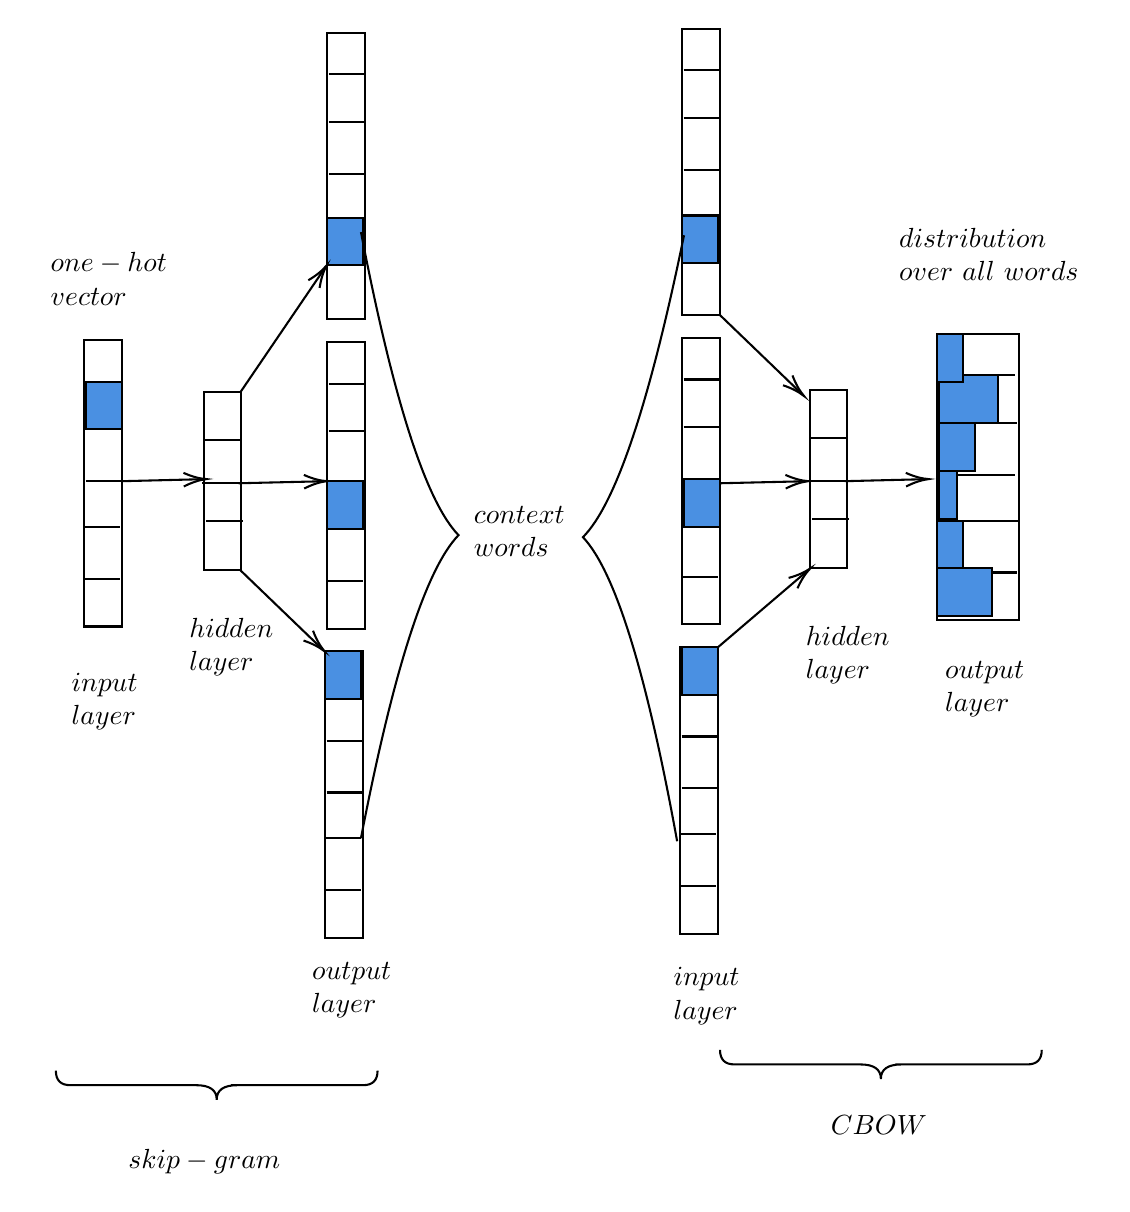
\begin{tikzpicture}[x=0.75pt,y=0.75pt,yscale=-1,xscale=1]
%uncomment if require: \path (0,608); %set diagram left start at 0, and has height of 608

%Shape: Rectangle [id:dp3485846016801524] 
\draw   (32,156) -- (50.5,156) -- (50.5,294) -- (32,294) -- cycle ;
%Shape: Rectangle [id:dp8456709052048703] 
\draw   (90,181) -- (107.5,181) -- (107.5,267) -- (90,267) -- cycle ;
%Straight Lines [id:da261980941990962] 
\draw    (33,176) -- (50.5,176) ;


%Straight Lines [id:da2112077987204617] 
\draw    (33,199) -- (50.5,199) ;


%Straight Lines [id:da8306488203565181] 
\draw    (33,224) -- (50.5,224) ;


%Straight Lines [id:da2601610712460867] 
\draw    (32,246) -- (49.5,246) ;


%Straight Lines [id:da5238964279791503] 
\draw    (32,271) -- (49.5,271) ;


%Straight Lines [id:da8696264510823728] 
\draw    (90,204) -- (107.5,204) ;


%Straight Lines [id:da18281681508420422] 
\draw    (89,225) -- (106.5,225) ;


%Straight Lines [id:da7605537343893694] 
\draw    (91,243) -- (108.5,243) ;


%Shape: Rectangle [id:dp7179646823512316] 
\draw   (149,8) -- (167.5,8) -- (167.5,146) -- (149,146) -- cycle ;
%Straight Lines [id:da37315938965868667] 
\draw    (150,28) -- (167.5,28) ;


%Straight Lines [id:da17887383176459348] 
\draw    (150,51) -- (167.5,51) ;


%Straight Lines [id:da05916336325961158] 
\draw    (150,76) -- (167.5,76) ;


%Straight Lines [id:da5760610647676259] 
\draw    (149,98) -- (166.5,98) ;


%Straight Lines [id:da6528261772940696] 
\draw    (149,120) -- (166.5,120) ;


%Shape: Rectangle [id:dp8883127519205649] 
\draw   (149,157) -- (167.5,157) -- (167.5,295) -- (149,295) -- cycle ;
%Straight Lines [id:da06170003747009711] 
\draw    (150,177) -- (167.5,177) ;


%Straight Lines [id:da41536185218273225] 
\draw    (150,200) -- (167.5,200) ;


%Straight Lines [id:da42678869727576263] 
\draw    (150,225) -- (167.5,225) ;


%Straight Lines [id:da4310051753333286] 
\draw    (149,247) -- (166.5,247) ;


%Straight Lines [id:da053035267754805604] 
\draw    (149,272) -- (166.5,272) ;


%Shape: Rectangle [id:dp5517809725941882] 
\draw   (148,306) -- (166.5,306) -- (166.5,444) -- (148,444) -- cycle ;
%Straight Lines [id:da4185941337540897] 
\draw    (149,326) -- (166.5,326) ;


%Straight Lines [id:da47456328490948096] 
\draw    (149,349) -- (166.5,349) ;


%Straight Lines [id:da5901537425032239] 
\draw    (149,374) -- (166.5,374) ;


%Straight Lines [id:da7036154379064874] 
\draw    (148,396) -- (165.5,396) ;


%Straight Lines [id:da6994685341101832] 
\draw    (148,421) -- (165.5,421) ;


%Shape: Rectangle [id:dp45444568393843277] 
\draw  [fill={rgb, 255:red, 74; green, 144; blue, 226 }  ,fill opacity=1 ] (33,176) -- (50.5,176) -- (50.5,199) -- (33,199) -- cycle ;
%Shape: Rectangle [id:dp9503787207911663] 
\draw   (320,6) -- (338.5,6) -- (338.5,144) -- (320,144) -- cycle ;
%Straight Lines [id:da688505041830114] 
\draw    (321,26) -- (338.5,26) ;


%Straight Lines [id:da5052098342263427] 
\draw    (321,49) -- (338.5,49) ;


%Straight Lines [id:da6656042500287078] 
\draw    (321,74) -- (338.5,74) ;


%Straight Lines [id:da33259654701711194] 
\draw    (320,96) -- (337.5,96) ;


%Straight Lines [id:da18673831484362013] 
\draw    (320,118) -- (337.5,118) ;


%Shape: Rectangle [id:dp10900029703116032] 
\draw   (320,155) -- (338.5,155) -- (338.5,293) -- (320,293) -- cycle ;
%Straight Lines [id:da6085648018600536] 
\draw    (321,175) -- (338.5,175) ;


%Straight Lines [id:da39621286199163275] 
\draw    (321,198) -- (338.5,198) ;


%Straight Lines [id:da4397876069903339] 
\draw    (321,223) -- (338.5,223) ;


%Straight Lines [id:da9804654346229789] 
\draw    (320,245) -- (337.5,245) ;


%Straight Lines [id:da4950448346788461] 
\draw    (320,270) -- (337.5,270) ;


%Shape: Rectangle [id:dp9790933731899871] 
\draw   (319,304) -- (337.5,304) -- (337.5,442) -- (319,442) -- cycle ;
%Straight Lines [id:da35864652577523115] 
\draw    (320,324) -- (337.5,324) ;


%Straight Lines [id:da7495817398749027] 
\draw    (320,347) -- (337.5,347) ;


%Straight Lines [id:da7414610589054373] 
\draw    (320,372) -- (337.5,372) ;


%Straight Lines [id:da30481781875545044] 
\draw    (319,394) -- (336.5,394) ;


%Straight Lines [id:da6933238629852232] 
\draw    (319,419) -- (336.5,419) ;


%Shape: Rectangle [id:dp41599720784303096] 
\draw   (382,180) -- (399.5,180) -- (399.5,266) -- (382,266) -- cycle ;
%Straight Lines [id:da5197607259717696] 
\draw    (382,203) -- (399.5,203) ;


%Straight Lines [id:da0670069440192731] 
\draw    (381,224) -- (398.5,224) ;


%Straight Lines [id:da8985276995166511] 
\draw    (383,242) -- (400.5,242) ;


%Shape: Rectangle [id:dp682541531707082] 
\draw   (443,153) -- (482.5,153) -- (482.5,291) -- (443,291) -- cycle ;
%Straight Lines [id:da6869201222736403] 
\draw    (444,173) -- (480.5,173) ;


%Straight Lines [id:da712489566777907] 
\draw    (444,196) -- (481.5,196) ;


%Straight Lines [id:da5319045187729963] 
\draw    (444,221) -- (480.5,221) ;


%Straight Lines [id:da05122157968239449] 
\draw    (443,243) -- (482.5,243) ;


%Straight Lines [id:da83248666674219] 
\draw    (443,268) -- (481.5,268) ;


%Shape: Rectangle [id:dp030697412111592826] 
\draw  [fill={rgb, 255:red, 74; green, 144; blue, 226 }  ,fill opacity=1 ] (149,97) -- (166.5,97) -- (166.5,120) -- (149,120) -- cycle ;
%Shape: Rectangle [id:dp7365845250356775] 
\draw  [fill={rgb, 255:red, 74; green, 144; blue, 226 }  ,fill opacity=1 ] (149,224) -- (166.5,224) -- (166.5,247) -- (149,247) -- cycle ;
%Shape: Rectangle [id:dp2882364519741776] 
\draw  [fill={rgb, 255:red, 74; green, 144; blue, 226 }  ,fill opacity=1 ] (148,306) -- (165.5,306) -- (165.5,329) -- (148,329) -- cycle ;
%Shape: Rectangle [id:dp7948565026182086] 
\draw  [fill={rgb, 255:red, 74; green, 144; blue, 226 }  ,fill opacity=1 ] (321,223) -- (338.5,223) -- (338.5,246) -- (321,246) -- cycle ;
%Shape: Rectangle [id:dp2733083899440938] 
\draw  [fill={rgb, 255:red, 74; green, 144; blue, 226 }  ,fill opacity=1 ] (320,96) -- (337.5,96) -- (337.5,119) -- (320,119) -- cycle ;
%Shape: Rectangle [id:dp4443146955310082] 
\draw  [fill={rgb, 255:red, 74; green, 144; blue, 226 }  ,fill opacity=1 ] (320,304) -- (337.5,304) -- (337.5,327) -- (320,327) -- cycle ;
%Shape: Rectangle [id:dp5065000833633793] 
\draw  [fill={rgb, 255:red, 74; green, 144; blue, 226 }  ,fill opacity=1 ] (444,173) -- (472.5,173) -- (472.5,196) -- (444,196) -- cycle ;
%Shape: Rectangle [id:dp1943242112575747] 
\draw  [fill={rgb, 255:red, 74; green, 144; blue, 226 }  ,fill opacity=1 ] (444,196) -- (461.5,196) -- (461.5,219) -- (444,219) -- cycle ;
%Shape: Rectangle [id:dp7118602383225767] 
\draw  [fill={rgb, 255:red, 74; green, 144; blue, 226 }  ,fill opacity=1 ] (443,243) -- (455.5,243) -- (455.5,266) -- (443,266) -- cycle ;
%Shape: Rectangle [id:dp3500880693070776] 
\draw  [fill={rgb, 255:red, 74; green, 144; blue, 226 }  ,fill opacity=1 ] (443,153) -- (455.5,153) -- (455.5,176) -- (443,176) -- cycle ;
%Shape: Rectangle [id:dp678028017987337] 
\draw  [fill={rgb, 255:red, 74; green, 144; blue, 226 }  ,fill opacity=1 ] (443,266) -- (469.5,266) -- (469.5,289) -- (443,289) -- cycle ;
%Shape: Rectangle [id:dp9868604783555972] 
\draw  [fill={rgb, 255:red, 74; green, 144; blue, 226 }  ,fill opacity=1 ] (444,219) -- (452.5,219) -- (452.5,242) -- (444,242) -- cycle ;
%Straight Lines [id:da7404729622737669] 
\draw    (50.5,224) -- (89,223.05) ;
\draw [shift={(91,223)}, rotate = 538.5899999999999] [color={rgb, 255:red, 0; green, 0; blue, 0 }  ][line width=0.75]    (10.93,-3.29) .. controls (6.95,-1.4) and (3.31,-0.3) .. (0,0) .. controls (3.31,0.3) and (6.95,1.4) .. (10.93,3.29)   ;

%Straight Lines [id:da9902030193329787] 
\draw    (398.5,224) -- (437,223.05) ;
\draw [shift={(439,223)}, rotate = 538.5899999999999] [color={rgb, 255:red, 0; green, 0; blue, 0 }  ][line width=0.75]    (10.93,-3.29) .. controls (6.95,-1.4) and (3.31,-0.3) .. (0,0) .. controls (3.31,0.3) and (6.95,1.4) .. (10.93,3.29)   ;

%Straight Lines [id:da44724706623553967] 
\draw    (107.5,181) -- (147.88,121.65) ;
\draw [shift={(149,120)}, rotate = 484.23] [color={rgb, 255:red, 0; green, 0; blue, 0 }  ][line width=0.75]    (10.93,-3.29) .. controls (6.95,-1.4) and (3.31,-0.3) .. (0,0) .. controls (3.31,0.3) and (6.95,1.4) .. (10.93,3.29)   ;

%Straight Lines [id:da6591012419225488] 
\draw    (106.5,225) -- (147,224.05) ;
\draw [shift={(149,224)}, rotate = 538.65] [color={rgb, 255:red, 0; green, 0; blue, 0 }  ][line width=0.75]    (10.93,-3.29) .. controls (6.95,-1.4) and (3.31,-0.3) .. (0,0) .. controls (3.31,0.3) and (6.95,1.4) .. (10.93,3.29)   ;

%Straight Lines [id:da5440847897108609] 
\draw    (107.5,267) -- (146.56,304.61) ;
\draw [shift={(148,306)}, rotate = 223.92000000000002] [color={rgb, 255:red, 0; green, 0; blue, 0 }  ][line width=0.75]    (10.93,-3.29) .. controls (6.95,-1.4) and (3.31,-0.3) .. (0,0) .. controls (3.31,0.3) and (6.95,1.4) .. (10.93,3.29)   ;

%Straight Lines [id:da5190845621462998] 
\draw    (338.5,144) -- (377.56,181.61) ;
\draw [shift={(379,183)}, rotate = 223.92000000000002] [color={rgb, 255:red, 0; green, 0; blue, 0 }  ][line width=0.75]    (10.93,-3.29) .. controls (6.95,-1.4) and (3.31,-0.3) .. (0,0) .. controls (3.31,0.3) and (6.95,1.4) .. (10.93,3.29)   ;

%Straight Lines [id:da47512326293326446] 
\draw    (337.5,304) -- (380.48,267.3) ;
\draw [shift={(382,266)}, rotate = 499.5] [color={rgb, 255:red, 0; green, 0; blue, 0 }  ][line width=0.75]    (10.93,-3.29) .. controls (6.95,-1.4) and (3.31,-0.3) .. (0,0) .. controls (3.31,0.3) and (6.95,1.4) .. (10.93,3.29)   ;

%Straight Lines [id:da8764420604284149] 
\draw    (338.5,225) -- (379,224.05) ;
\draw [shift={(381,224)}, rotate = 538.65] [color={rgb, 255:red, 0; green, 0; blue, 0 }  ][line width=0.75]    (10.93,-3.29) .. controls (6.95,-1.4) and (3.31,-0.3) .. (0,0) .. controls (3.31,0.3) and (6.95,1.4) .. (10.93,3.29)   ;

%Shape: Brace [id:dp39390698992163764] 
\draw   (18.5,508) .. controls (18.5,512.67) and (20.83,515) .. (25.5,515) -- (86,515) .. controls (92.67,515) and (96,517.33) .. (96,522) .. controls (96,517.33) and (99.33,515) .. (106,515)(103,515) -- (166.5,515) .. controls (171.17,515) and (173.5,512.67) .. (173.5,508) ;
%Shape: Brace [id:dp01887132985159412] 
\draw   (338.5,498) .. controls (338.5,502.67) and (340.83,505) .. (345.5,505) -- (406,505) .. controls (412.67,505) and (416,507.33) .. (416,512) .. controls (416,507.33) and (419.33,505) .. (426,505)(423,505) -- (486.5,505) .. controls (491.17,505) and (493.5,502.67) .. (493.5,498) ;
\draw   (165.5,104) .. controls (181.17,185.11) and (196.83,233.78) .. (212.5,250) .. controls (196.83,266.22) and (181.17,314.89) .. (165.5,396) ;
\draw   (317.84,397.5) .. controls (303.08,316.22) and (287.95,267.38) .. (272.45,250.98) .. controls (288.32,234.93) and (304.55,186.45) .. (321.15,105.52) ;

% Text Node
\draw (466,324) node   {$ \begin{array}{l}
output\\
layer
\end{array}$};
% Text Node
\draw (161,469) node   {$ \begin{array}{l}
output\\
layer
\end{array}$};
% Text Node
\draw (332,472) node   {$ \begin{array}{l}
input\\
layer
\end{array}$};
% Text Node
\draw (42,330) node   {$ \begin{array}{l}
input\\
layer
\end{array}$};
% Text Node
\draw (400,308) node   {$ \begin{array}{l}
hidden\\
layer
\end{array}$};
% Text Node
\draw (103,304) node   {$ \begin{array}{l}
hidden\\
layer
\end{array}$};
% Text Node
\draw (44,128) node   {$ \begin{array}{l}
one-hot\\
vector
\end{array}$};
% Text Node
\draw (90,552) node   {$skip-gram$};
% Text Node
\draw (415,534) node   {$CBOW$};
% Text Node
\draw (244,249) node   {$ \begin{array}{l}
context\ \\
words
\end{array}$};
% Text Node
\draw (468,116) node   {$ \begin{array}{l}
distribution\\
over\ all\ words
\end{array}$};


\end{tikzpicture}




\tikzset{every picture/.style={line width=0.75pt}} %set default line width to 0.75pt        

\begin{tikzpicture}[x=0.75pt,y=0.75pt,yscale=-1,xscale=1]
%uncomment if require: \path (0,300); %set diagram left start at 0, and has height of 300





\end{tikzpicture}



}
\caption{Predict a word, given the preceding and following words (Continuous Bag of Words, CBOW) and predict the preceding and following words, given a word (Skip-Gram). Image inspired by~\brackettext{\cite{DBLP:journals/corr/abs-1301-3781}}.}
\label{fig:w2v}
\end{figure}
%%%%%%%%%%%%%%%%%%%%%%%%%%%%%%%%%%%%%%%%%%%%%%%%%%%%%%%%%%%%
\subsection{Word2vec: Distributed representations of words}
\label{subsec:word2vec}
The goal of word2vec model is, given a center word, to predict the words that occur in its surroundings. If sufficient data is used for training, word2vec can predict with high accuracy the word's meaning based on its surrounding words in the corpus and also successfully capture semantic relations, such as country and capital relations, as well as syntactic relations. For example, the vector representation of  \emph{``man''} has approximately the same distance to \emph{``brother''} as \emph{``women''} to \emph{``sister''}. \\
The word2vec method contains two models, the \emph{continuous bag-of-words} (CBOW) and the \emph{skip-gram} architecture. Both are shown in Figure~\ref{fig:w2v}. The CBOW architecture predicts the current word-based on the context and the skip-gram predicts surrounding words given the current word. While the two models are quite similar, they have different attributes. The CBOW smooths over a lot of the distributional information (by treating an entire context as one observation), which makes it useful for smaller datasets. However, skip-gram treats each context-target pair as a new observation and tends to do better on the larger datasets~\brackettext{\cite{DBLP:journals/corr/MandelbaumS16}}. In the following, we will focus on the skip-gram model. \\
\begin{figure}
\centering 
\resizebox{0.8\textwidth}{0.5\textwidth}{      
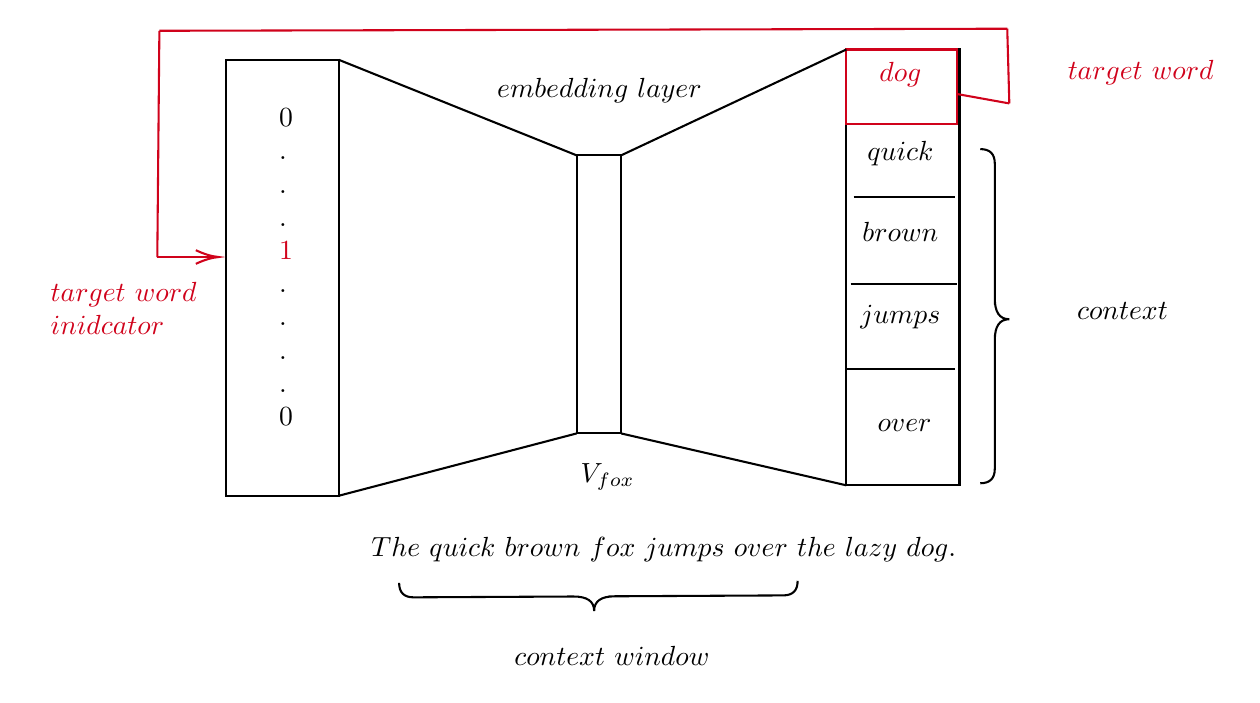
\begin{tikzpicture}[x=0.75pt,y=0.75pt,yscale=-1,xscale=1]
%uncomment if require: \path (0,347); %set diagram left start at 0, and has height of 347

%Shape: Rectangle [id:dp34856826620420023] 
\draw   (288,66) -- (309.5,66) -- (309.5,200) -- (288,200) -- cycle ;
%Shape: Rectangle [id:dp20385411601802828] 
\draw   (418,15) -- (472.5,15) -- (472.5,225) -- (418,225) -- cycle ;
%Shape: Rectangle [id:dp597929679831426] 
\draw  [color={rgb, 255:red, 208; green, 2; blue, 27 }  ,draw opacity=1 ] (418,15) -- (471.5,15) -- (471.5,51) -- (418,51) -- cycle ;
%Straight Lines [id:da329141353304766] 
\draw    (421.5,86) -- (470.5,86) ;


%Shape: Brace [id:dp7412735560954036] 
\draw   (202.5,272) .. controls (202.53,276.67) and (204.87,278.99) .. (209.54,278.96) -- (286.44,278.56) .. controls (293.11,278.53) and (296.45,280.84) .. (296.48,285.51) .. controls (296.45,280.84) and (299.77,278.49) .. (306.44,278.46)(303.44,278.47) -- (387.54,278.03) .. controls (392.21,278) and (394.53,275.66) .. (394.5,270.99) ;
%Straight Lines [id:da1987933863065281] 
\draw    (420,128) -- (471.5,128) ;


%Straight Lines [id:da8961013192322056] 
\draw    (418.5,169) -- (470.5,169) ;


%Shape: Brace [id:dp8413236825652046] 
\draw   (482.5,224) .. controls (487.17,224) and (489.5,221.67) .. (489.5,217) -- (489.5,154.97) .. controls (489.5,148.3) and (491.83,144.97) .. (496.5,144.97) .. controls (491.83,144.97) and (489.5,141.64) .. (489.5,134.97)(489.5,137.97) -- (489.5,70) .. controls (489.5,65.33) and (487.17,63) .. (482.5,63) ;
%Shape: Rectangle [id:dp5223635802427213] 
\draw   (119,20) -- (173.5,20) -- (173.5,230) -- (119,230) -- cycle ;
%Straight Lines [id:da26424324688833556] 
\draw [color={rgb, 255:red, 208; green, 2; blue, 27 }  ,draw opacity=1 ]   (86,115) -- (113.5,115) ;
\draw [shift={(115.5,115)}, rotate = 180] [color={rgb, 255:red, 208; green, 2; blue, 27 }  ,draw opacity=1 ][line width=0.75]    (10.93,-3.29) .. controls (6.95,-1.4) and (3.31,-0.3) .. (0,0) .. controls (3.31,0.3) and (6.95,1.4) .. (10.93,3.29)   ;

%Straight Lines [id:da3427921645180725] 
\draw [color={rgb, 255:red, 208; green, 2; blue, 27 }  ,draw opacity=1 ]   (87,6) -- (86,115) ;


%Straight Lines [id:da5378893688694539] 
\draw [color={rgb, 255:red, 208; green, 2; blue, 27 }  ,draw opacity=1 ]   (87,6) -- (495.5,5) ;


%Straight Lines [id:da1316572119067576] 
\draw [color={rgb, 255:red, 208; green, 2; blue, 27 }  ,draw opacity=1 ]   (495.5,5) -- (496.5,41) ;


%Straight Lines [id:da7079049036395544] 
\draw [color={rgb, 255:red, 208; green, 2; blue, 27 }  ,draw opacity=1 ]   (471.5,36.5) -- (496.5,41) ;


%Straight Lines [id:da6232994776605181] 
\draw    (173.5,20) -- (288,66) ;


%Straight Lines [id:da1671416061216935] 
\draw    (173.5,230) -- (288,200) ;


%Straight Lines [id:da8246799797542117] 
\draw    (309.5,66) -- (418,15) ;


%Straight Lines [id:da7881561473504775] 
\draw    (309.5,200) -- (418,225) ;



% Text Node
\draw (330,256) node   {$The\ quick\ brown\ fox\ jumps\ over\ the\ lazy\ dog.$};
% Text Node
\draw (303,221) node   {$V_{fox}$};
% Text Node
\draw (299,35) node   {$embedding\ layer$};
% Text Node
\draw (562,26) node [color={rgb, 255:red, 208; green, 2; blue, 27 }  ,opacity=1 ]  {$target\ word\ $};
% Text Node
\draw (444,27) node [color={rgb, 255:red, 208; green, 2; blue, 27 }  ,opacity=1 ]  {$dog$};
% Text Node
\draw (444,65) node   {$quick$};
% Text Node
\draw (444,103) node   {$brown$};
% Text Node
\draw (444,144) node   {$jumps$};
% Text Node
\draw (446,196) node   {$over$};
% Text Node
\draw (551,141) node   {$context$};
% Text Node
\draw (305,307) node   {$context\ window$};
% Text Node
\draw (148,121) node   {$ \begin{array}{l}
0\\
.\\
.\\
.\\
\textcolor[rgb]{0.82,0.01,0.11}{1}\\
.\\
.\\
.\\
.\\
0
\end{array}$};
% Text Node
\draw (72,141) node [color={rgb, 255:red, 208; green, 2; blue, 27 }  ,opacity=1 ]  {$ \begin{array}{l}
target\ word\ \\
inidcator
\end{array}$};


\end{tikzpicture}

}
\caption{Skip-gram architecture for the example sentence \emph{``The quick brown fox jumps over the lazy dog.''}. The input is the one-hot vector indicating the word \emph{``dog''} and the model tries to predict words that co-occur in the context window of the target word.  }
\label{fig:skip_w2v}
\end{figure}
\noindent
The skip-gram objective is to train word vector representations that are good at predicting the nearby words. A visual representation of the skip-gram model can be seen in Figure~\ref{fig:skip_w2v} for the sentence \emph{``The quick brown fox jumps over the lazy dog.''}, where the meaning of the word \emph{``fox''} is defined by the words in the window around it. The input is the one-hot vector for the the target word and the output is the context words.\\
More formally, given a corpus of target words $f$ and their contexts $c$, the goal is to learn the parameter $w$ of $p(c|f; w)$, so as to maximize the corpus probability, where $Q$ is the set of all words and context pairs extracted from the text. Equation~\ref{eq:w2v_p} shows the probability formulation.
\begin{equation}
\label{eq:w2v_p}
w^*=\underset { w  }{ { \text{argmax} } } \prod _{ (w,c)\in Q }^{  }{ p(c|f;  w )}
\end{equation}
The literature on neural-network language models, defines this probability using softmax shown in Equation~\ref{eq:w2v_softmax}, where $w_c$ and $ w_f\in R^d$ are vector representations for $c$ (context words) and $f$ (focal or center word) respectively, and
$C$ is the set of all available contexts. The goal is to find the parameter $w$ such that Equation~\ref{eq:w2v_p} is maximized~\brackettext{\cite{DBLP:journals/corr/GoldbergL14}}. 
\begin{equation}
\label{eq:w2v_softmax}
p(c|f;w)=\frac { { e }^{ w_{ c }.w_{ f } } }{ \sum _{ \overline { f } \in C }^{  }{ { e }^{ w_{ c }.w_{ \overline { f }  } } }  } 
\end{equation}
Maximizing the log-likelihood of Equation~\ref{eq:w2v_softmax} on the training set is very expensive. Because we need to compute and normalize each probability using the score for all other words  $\overline { f }$ in the context of $c$. Therefore, the authors reformulate the problem using \emph{Negative Sampling}~\brackettext{\cite{DBLP:journals/jmlr/GutmannH12}}. Negative sampling is used in order to deal with the expensive computation of the softmax, in which the multinomial classification problem (predicting the next word) is converted into a binary classification problem. To estimate a true probability distribution of the output word, binary logistic regression is used, where the classifier learns to distinguish between a true pair (true context words) and randomly selected words from the vocabulary (corrupted pairs). The classifier simply predicts whether a pair of words is a true or a random sample. The new objective function, using negative sampling, is shown in Equation~\ref{eq:w2v_negative}. $ \sigma$ shows the sigmoid function and $\overline{Q}$ is the set of random $(f, c)$ pairs, assuming they are all incorrect. By maximizing this objective, the model assigns high probabilities to the real word pairs, and low probabilities to noise word pairs. Furthermore, it is more computationally appealing than the softmax function.

\begin{equation}
\label{eq:w2v_negative}
\underset { w }{ \mathrm{ argmax } } \sum _{ (c,a)\in Q }^{  }{ \log { \sigma ( } w_{ c }.w_{ f }) } +\sum _{ (c,\overline {f})\in \overline { Q }  }^{  }{ \log { \sigma ( } -w_{ c }.w_{ \overline {f} })\quad  } 
\end{equation}
If the model is trained on enough data, word2vec groups the vectors of similar words together in vector space, finds word’s associations and detects similarities mathematically with cosine similarity. 
%%%%%%%%%%%%%%%%%%%%%%%%%%%%%%%%%%%%%%%%%%%%%%%%%%%%%%%%%%%%
\subsection{GloVe: Global vector embeddings}
\label{subsec:GloVe}
The \emph{Global Vector Model} (GloVe) suggests that the ratio of co-occurrence probabilities can encode meaning components. An example can be seen in Table~\ref{table:tab_1}, in terms of studying a thermodynamic phase. A meaning component that sets the word \emph{``ice''} apart from \emph{``steam''} is represented as a ratio of their occurrence probability with all other words \big($\frac { P(ice|k) }{ P(steam|k) } $, where $k$ can be any word in the vocabulary\big). This ratio can distinguish relevant words in comparison from irrelevant ones by giving the irrelevant ones a probability close to one. Also compared to the raw probabilities, it is better able to discriminate between the relevant words by giving the relevant ones a high ratio, such as words like \emph{``solid''}, and low ratio to irrelevant ones, such as \emph{``gas''}. As a result, the word \emph{``ice''} stand out as a solid object. Moreover, words, such as \emph{``water''} or \emph{``fashion''}, therefore, has a probability close to one as it is either a shared property or not related to the concept.\\
\begin{table}[]
\centering

\begin{tabular}{@{}l|l|l|l|l@{}}
\toprule
Probability and Ratio &  $k=solid$& $k=gas$ & $k=water$ &$k= fashion$  \\ \midrule $P(k|ice)$& {\color[HTML]{CB0000}large} &  {\color[HTML]{329A9D}small} & {\color[HTML]{CB0000}large} & {\color[HTML]{329A9D}small} \\\midrule
  $P(k|steam)$&{\color[HTML]{329A9D}small}  & {\color[HTML]{CB0000}large} &  {\color[HTML]{CB0000}large}&{\color[HTML]{329A9D}small}  \\\midrule
 $\frac { P(ice|k) }{ P(steam|k) } $& {\color[HTML]{CB0000}large} &  {\color[HTML]{329A9D}small}&  1 &    1  \\\midrule
\end{tabular}%
\caption{Co-occurrence probabilities for target words \emph{``ice''}and \emph{``steam''} with selected context words. Example taken from~\brackettext{\cite{DBLP:conf/emnlp/PenningtonSM14}}.}
\label{table:tab_1}
\end{table}
\noindent
To capture these ratios, the authors of GloVe propose a log-bilinear model, where, if the dot product of two vectors corresponds to the log of their co-occurrence probability, their difference will show the meaning component. The relation of the dot product of the word embeddings with the co-occurrence probability, for two word $i$ and $j$, based on assumptions of the GloVe model is shown in Equation~\ref{eq:log_prob}, where $w_i$ is the word embedding for the word $i$. 
\begin{equation}
\begin{split}
\\ w_{ i }.w_{ j }=\log { P(i|j)\quad  } \\
w_{ x }(w_{ i }-w_{ j })=\log { \frac { P(x|j) }{ P(x|j) } } 
\end{split}
\label{eq:log_prob}
\end{equation}
Let the matrix of word-word co-occurrence counts be denoted by $X\in { R }^{ |V|\times |V| }$, where $|V|$ is the size of the vocabulary.  Entries $X_{fc}$ tabulate the number of times word $c$ occurs in the context of word $f$. $w_{ f }\in { R }^{ 1\times M }$ and $\tilde{w_{ c }}\in { R }^{ 1\times M }$ are the focal (center word) and context embeddings, respectively, where $M$ is the embedding size. The model tries to learn embeddings that minimize the squared difference between the dot product of the center and context word embedding and the logarithm of their co-occurrence count.
Considering $ \tilde{b_{ f }}$ and $b_{ c }$  as the biases for the focal and context embeddings, the cost function is defined in Equation~\ref{eq:glove_cost}. Since the log of co-occurrences does not directly result in a probability, in order for the meaning component to have a probabilistic interpretation, a normalization factor is needed. Bias $b_{ f }$ allows the model to learn this constant during training and $ \tilde{b_{ c }}$ is added to preserve symmetry. 
\begin{equation}
J=\sum _{ f,c=1 }^{ |V| }{ f({ X }_{ fc } } )(w_{ f }^{ \top }\tilde{  w_{ c } } +b_{ f }+\tilde{  b_{ c } } -\log{ X }_{ fc })^2
\label{eq:glove_cost}
\end{equation}
optimising for the co-occurrence counts alone might cause the model to overemphasize the most common words. Therefore, a weighting function ($f$) is introduced that imposes an upper bound on the maximum number of co-occurrences between two words. Conceptually, $f$ scales the counts in order to avoid the influence of common words and boost the rare words. The choice of $f$ is not fixed, but one class of functions that is used by the authors is parametrized with $\alpha$ as the exponential weight and $x_{max}$ as the maximum number of allowed co-occurrences. $\alpha$ and $x_{max}$ are hyper-parameters that require tuning, but the values suggested by the authors are $\frac{3}{4}$ for $\alpha$ is  and $100$ for $x_{max}$. 
\begin{equation}
f=\left\{
  \begin{array}{@{}ll@{}}
    (\frac { x }{ { x }_{ \max } } )^{ \alpha  }& \text{if}\ x<x_{max} \\
    1 & \text{otherwise}
  \end{array}\right.
\label{eq:weighingfunction}
\end{equation}
\noindent
The model learns two embeddings for each word, one as a focal or center word and the other as a context word. As the co-occurrence matrix is symmetric both of which can be considered as learning the same representation. Ultimately, the two embeddings are added to obtain the final embedding.
%%%%%%%%%%%%%%%%%%%%%%%%%%%%%%%%%%%%%%%%%%%%%%%%%%%%%%%%%%%%
\subsection{Similarity between embeddings}\label{sec:similarity}
The dense word vector representation is learned to capture the semantics of a word, and hence, similar words are close in the induced space. \emph{Cosine similarity} helps to capture this semantic closeness and is the most common similarity measure for  word vectors. The cosine similarity is a measure that calculates the cosine of the angle between two vectors. This metric is a measurement of orientation and not magnitude and it is derived from the equation of a dot product between two vectors, as shown in Equation~\ref{eq:cosine}. The vectors are normalized by their length, which removes the influence of their magnitude on the similarity. The norm of the vector is somewhat related to the overall frequency of which words occur in the training corpus, but the direction is unaffected by this. For similarity between two words, it is often the direction that matters and not the overall frequency in the corpus. So in order for a common word like \emph{``frog''} to still be similar to a less frequent word like \emph{``Anura''} (a type of frog), cosine similarity which only looks at the direction works better than simple Euclidean distance. Moreover, cosine similarity is symmetric and therefore, changing the order of vectors in the dot product does not affect the final result.
\begin{equation}
\begin{split}
\overrightarrow { w_i } .\overrightarrow { w_j } =\parallel \overrightarrow { w_i } \parallel \parallel \overrightarrow { w_j } \parallel cos\theta 
\\
cos\theta =\frac { \overrightarrow { w_i } .\overrightarrow { w_j }  }{ \parallel \overrightarrow { w_i } \parallel \parallel \overrightarrow { w_j } \parallel  } 
\end{split}
\label{eq:cosine}
\end{equation}
%%%%%%%%%%%%%%%%%%%%%%%%%%%%%%%%%%%%%%%%%%%%%%%%%%%%%%%%%%%%
\subsection{Edge weights and co-occurrence probabilities}\label{subsec:weights_load}
The cost function of the GloVe model is based on the assumption that the ratio of co-occurrence probabilities results in meaningful components, which can be investigated to find the relation between two words. Edge weights of the LOAD model have a correlation with the co-occurrence counts of terms and entities in text. However, the sentence distance is a more efficient way to define a distance metric between two entities rather than a window-based approach. Two entities appearing in the same document tend to have some connection, this relationship is disregarded if we only look at a small window of words. Additionally, since the weights decay based on how far an entity is from another, we gain more information about the structure of the text. Based on these considerations, we argue that LOAD edge weights produce a better overall corpus statistics in case of named entities in comparison to a simple co-occurrence matrix and that it can generate the same meaningful components like probability ratios. \\
\begin{table}[]
\centering

\begin{tabular}{@{}l|l|l|l|l@{}}
\toprule
Probability and Ratio&  $k=republican$& $k=democratic$ & $k=president$ &$k= BMW$  \\ \midrule
 $P(k|Trump)$& {\color[HTML]{CB0000}10.51} &  {\color[HTML]{329A9D}5.30} & {\color[HTML]{CB0000}52} & {\color[HTML]{329A9D}0} \\\midrule
  $P(k|Obama)$&{\color[HTML]{329A9D}0.36}  & {\color[HTML]{CB0000}1.29} &  {\color[HTML]{CB0000}66}&{\color[HTML]{329A9D}0}  \\\midrule
 $\frac { P(Trump|k) }{ P(Obama|k) } $& {\color[HTML]{CB0000}29.2} &  {\color[HTML]{329A9D}4.10}&  0.78 &    0  \\\midrule
\end{tabular}%

\caption{LOAD weights for target words \emph{``Donald Trump''} and \emph{``Barack Obama''} with selected context words. }
\label{table:tab_2}
\end{table}
\label{sec:components_load}
We demonstrate this claim with a simple example in Table~\ref{table:tab_2} that shows how certain aspects of meaning can be extracted from edge weights of LOAD. Suppose we are interested in the concept of US presidents, for which we take two actors \emph{``Donald Trump''} and \emph{``Barack Obama''}. The relationship between these entities is examined by studying the ratio of their edge weights with various probe words. Similar to the GloVe model, where the ratio of co-occurrence probability distinguished the relevant words from irrelevant words, here the ratio of the edge weights works in the same way. In this case, looking at the raw edge weights does not give us much comparable information, but the ratio denotes \emph{``Donald Trump''} as a republican rather than a democratic politician. Since both of the entities share the presidential attribute the ratio is close to one. On the other hand, a random name like \emph{``BMW''} has a relatively small weight with both entities, but since the weak edges were cut off from the model we have the weight of zero. If  the full graph without a cut-off threshold is considered instead, the ratio of two small numbers will also converge to one, implying that similar to co-occurrence matrix, edge weights of LOAD produce meaning components. As a result, the bilinearity assumption of GloVe can be extended to the weighted adjacency matrix of LOAD. 

%%%%%%%%%%%%%%%%%%%%%%%%%%%%%%%%%%%%%%%%%%%%%%%%%%%%%%%%%%%%
\section{Entity Embeddings}
\label{sec:enity_embed}
Entity embedding are mostly studied in the context of embedding knowledge graphs in prepration of a downstream task, usually for entity disambiguation. Guo and Barbosa use random walks on knowledge graphs to construct vector representations of entities for named entity disambiguation task~\brackettext{\cite{DBLP:journals/semweb/GuoB18}}. He et al. use a deep neural network to represent the entities and their relations in knowledge graphs for inference tasks and link prediction in knowladge bases~\brackettext{\cite{DBLP:journals/corr/YangYHGD14a}}. Aside from pure knowledge graph embedding, a few models focus on combining word embeddings with embeddings from knowledge graphs for enity disambiguation tasks. In a paper by Yamada et al., the skip-gram model trained on a textual corpus is combined with knowledge graph embeddings, where the vectors are aligned, such that similar words and entities occur close to one another in the vector space. The learned embeddings are then used as a feature for named entity disambiguation~\brackettext{\cite{DBLP:conf/conll/YamadaS0T16}}. Fang et al. also take a similar approach and by learning word embeddings from text and entity embeddings from a knowledge graph. They use an alignment model that guarantees the vectors of entities and words are in the same space and utilize them to design features for their disambiguation framework~\brackettext{\cite{DBLP:conf/conll/FangZWCL16}}. All of the above methods, although successful at representing entities and words are dependent on knowledge bases as an extra source of information and often optimise different objective functions for learning the entity and word embeddings, or train them separately and combine them in a later step. In this thesis, we avoid using separate training objectives for entities and word and treat them equally to learn embeddings directly from annotated text. Furthermore, learning embeddings for words and entities simultaneously, removes the necessity for an extra alignment model. It is also important to note that since the above methods are designed as feature for a specific task, they are only evaluated through the performance on that task. In contrast, we focus on creating general-purpose entity embeddings that are comparable to normal word embeddings. Additionally, we evaluate our embeddings against state-of-the-art word embedding techniques to asses their advantages and drawbacks in performance. \\

%%%%%%%%%%%%%%%%%%%%%%%%%%%%%%%%%%%%%%%%%%%%%%%%%%%%%%%%%%%%
\section{Graph-based Embeddings}
\label{sec:graph}
Graph embeddings convert a graph into a low dimensional space in which the graph information is preserved. Therefore, it is an effective and efficient way to compute features from a graph for machine learning algorithms. Based on the embedding output, graph embeddings are categorized into four types: \emph{node embedding}, \emph{edge embedding}, \emph{hybrid embedding} (combination of different types of graph components, e.g., node $+$ edge), and  \emph{whole-graph embedding} (a graph is represented as one vector)~\brackettext{\cite{DBLP:journals/tkde/CaiZC18}}. In this thesis, we focus on node embedding, as we use it to extract entity embedding form a co-occurrence graph in later chatpers. Node embedding techqniques embed nodes of a graph in a low-dimensional vector that is usually smaller than the number of total number of nodes in the graph. Different node embedding models vary in their definition of similarity between nodes and the graph property they preserve. Two most important properties are \emph{first-order proximity} and \emph{second-order proximity}. First-order proximity captures the direct neighbourhood relationship (edges) in a graph. Second-order proximity captures the second step relations (number of common neighbours shared between two nodes). The second-order proximity can also be extended to take higher orders into account as well (third-order proximity and so on)~\brackettext{\cite{DBLP:journals/jmlr/GutmannH12}}.\\
Since the nodes of the co-occurrence graph correspond to words in the vocabulary, in this study we only look at node embedding techniques. Embedding the edges or whole graph does not provide any information about the words of the corpus. In the following we give a brief introduction into popular node embedding methods. 
%%%%%%%%%%%%%%%%%%%%%%%%%%%%%%%%%%%%%%%%%%%%%%%%%%%%%%%%%%%%
\subsection{DeepWalk, a random walk-based embedding}
\label{subsec:DeepWalk}
\begin{figure}
\centering 
\resizebox{0.8\textwidth}{0.35\textwidth}{      
\input{images/DeepWalk.tex}
}
\caption{The workflow of DeepWalk. It first generates random walk sequences from a graph, and then applies the skip-gram model to learn the embeddings. Figure adapted from~\brackettext{\cite{SCHOL:journal/IEEE/zahng}}.}
\label{fig:deepwalk}
\end{figure}

The \emph{DeepWalk}~\brackettext{\cite{DBLP:conf/kdd/PerozziAS14}} model learns latent representations of nodes of a graph using local information obtained from fixed length random walks. The model treats the nodes visited in the random walk as words and the walk itself as  a sentence from the corpus. Then the skip-gram is applied on the generated corpus to maximize the probability of visiting the neighbourhood of the node conditioned on its embedding. A visualization of the workflow of DeepWalk is shown in Figure~\ref{fig:deepwalk}. In other words, the model tries to learn the embedding $w\in R^{ d} $, where $d$ is a small number of latent dimensions in comparison to the number of nodes. The model maximizes the probability of observing the last $k$ nodes and the next $k$ nodes in the random walk entered at node $v_{i}$, by minimizing negative log of the probability as shown in the Equation~\ref{eq:dw}, to learn the node embedding $w$~\brackettext{\cite{DBLP:journals/kbs/GoyalF18}}.: 
\begin{equation}
J=-\log { P( } v_{ { i−k } },...,v_{ i−1 },v_{ i+1 },...,v_{ i+k }|w )
\label{eq:dw}
\end{equation}
Based on this approach, nodes that share similar neighbours in random walk sequences should be represented closely in the embedding space. Since the random walk in DeepWalk correspond to the \emph{Depth-first Sampling} (DFS) , it can preserve the second-order proximity. As a result, DeepWalk is good at keeping community structures. 
%%%%%%%%%%%%%%%%%%%%%%%%%%%%%%%%%%%%%%%%%%%%%%%%%%%%%%%%%%%%
\subsection{Node2vec: Scalable feature learning for graphs }
\label{subsec:node2vec}
\emph{Node2vec}~\brackettext{\cite{DBLP:conf/kdd/GroverL16}} extends the random walk procedure of DeepWalk by defining a more flexible notion of a node’s neighbourhood. There are mainly two node sampling strategies in random walk: \emph{Breadth-first Sampling} (BFS) and \emph{Depth-first Sampling} (DFS), where the BFS focuses on the immediate neighbours of the node and DFS consists of sampled nodes sequentially sampled at increasing distances from the source node~\brackettext{\cite{DBLP:conf/kdd/GroverL16}}.
Therefore, BFS represents the first-order proximity and DFS the second and higher-order proximity. A demonstration of different sampling methods is provided in Figure~\ref{fig:dfs_bfs}, where red arrows illustrated the BFS startegy and blue arrows show the DF startegy for a random walk with lenght $3$. Node2vec provides a trade-off between BFS and DFS sampling methods, with a use of two hyperparameters to regulate the balance between the them. By choosing a right balance between the two sampling methods, we preserve community structure as well as structural equivalence between nodes~\brackettext{\cite{DBLP:journals/kbs/GoyalF18}}.
Despite the flexiblity of node2vec, the method tends to be quite inefficient for large graphs and incurs significant space and time overhead. It runs out of memory even for mid-sized graphs, which is problematic for large co-occurrence graphs. Although there exist complex graph structures to speed up the process, the original model is very slow on large graphs ~\brackettext{\cite{DBLP:journals/corr/abs-1805-00280}}. 
\begin{figure}
\centering 
\resizebox{0.45\textwidth}{0.25\textwidth}{      
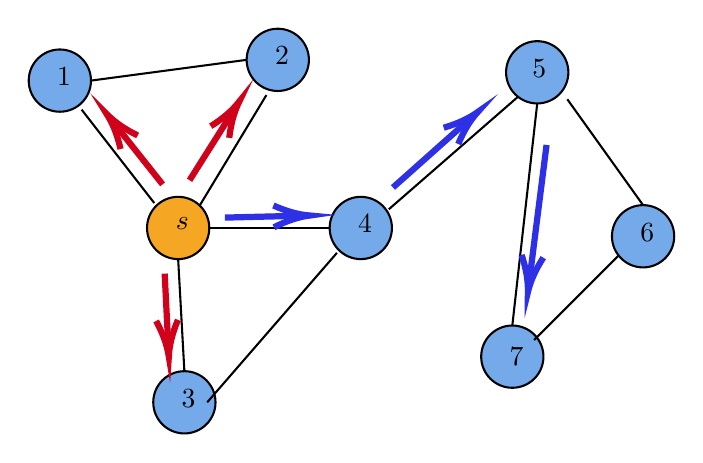
\begin{tikzpicture}[x=0.75pt,y=0.75pt,yscale=-1,xscale=1]
%uncomment if require: \path (0,407); %set diagram left start at 0, and has height of 407

%Shape: Circle [id:dp332493301566809] 
\draw  [fill={rgb, 255:red, 74; green, 144; blue, 226 }  ,fill opacity=0.77 ] (56,81) .. controls (56,72.72) and (62.72,66) .. (71,66) .. controls (79.28,66) and (86,72.72) .. (86,81) .. controls (86,89.28) and (79.28,96) .. (71,96) .. controls (62.72,96) and (56,89.28) .. (56,81) -- cycle ;
%Shape: Circle [id:dp4879070023914207] 
\draw  [fill={rgb, 255:red, 245; green, 166; blue, 35 }  ,fill opacity=1 ] (113,152) .. controls (113,143.72) and (119.72,137) .. (128,137) .. controls (136.28,137) and (143,143.72) .. (143,152) .. controls (143,160.28) and (136.28,167) .. (128,167) .. controls (119.72,167) and (113,160.28) .. (113,152) -- cycle ;
%Shape: Circle [id:dp5810034132491635] 
\draw  [fill={rgb, 255:red, 74; green, 144; blue, 226 }  ,fill opacity=0.77 ] (161,71) .. controls (161,62.72) and (167.72,56) .. (176,56) .. controls (184.28,56) and (191,62.72) .. (191,71) .. controls (191,79.28) and (184.28,86) .. (176,86) .. controls (167.72,86) and (161,79.28) .. (161,71) -- cycle ;
%Shape: Circle [id:dp678091001536465] 
\draw  [fill={rgb, 255:red, 74; green, 144; blue, 226 }  ,fill opacity=0.77 ] (116,236) .. controls (116,227.72) and (122.72,221) .. (131,221) .. controls (139.28,221) and (146,227.72) .. (146,236) .. controls (146,244.28) and (139.28,251) .. (131,251) .. controls (122.72,251) and (116,244.28) .. (116,236) -- cycle ;
%Shape: Circle [id:dp19856877490785307] 
\draw  [fill={rgb, 255:red, 74; green, 144; blue, 226 }  ,fill opacity=0.77 ] (201,152) .. controls (201,143.72) and (207.72,137) .. (216,137) .. controls (224.28,137) and (231,143.72) .. (231,152) .. controls (231,160.28) and (224.28,167) .. (216,167) .. controls (207.72,167) and (201,160.28) .. (201,152) -- cycle ;
%Shape: Circle [id:dp06052439820005162] 
\draw  [fill={rgb, 255:red, 74; green, 144; blue, 226 }  ,fill opacity=0.77 ] (286,77) .. controls (286,68.72) and (292.72,62) .. (301,62) .. controls (309.28,62) and (316,68.72) .. (316,77) .. controls (316,85.28) and (309.28,92) .. (301,92) .. controls (292.72,92) and (286,85.28) .. (286,77) -- cycle ;
%Shape: Circle [id:dp7842135850860721] 
\draw  [fill={rgb, 255:red, 74; green, 144; blue, 226 }  ,fill opacity=0.77 ] (274,214) .. controls (274,205.72) and (280.72,199) .. (289,199) .. controls (297.28,199) and (304,205.72) .. (304,214) .. controls (304,222.28) and (297.28,229) .. (289,229) .. controls (280.72,229) and (274,222.28) .. (274,214) -- cycle ;
%Shape: Circle [id:dp69600261549569] 
\draw  [fill={rgb, 255:red, 74; green, 144; blue, 226 }  ,fill opacity=0.77 ] (337,156) .. controls (337,147.72) and (343.72,141) .. (352,141) .. controls (360.28,141) and (367,147.72) .. (367,156) .. controls (367,164.28) and (360.28,171) .. (352,171) .. controls (343.72,171) and (337,164.28) .. (337,156) -- cycle ;
%Straight Lines [id:da49057224619926565] 
\draw    (81.5,95) -- (116.5,140) ;


%Straight Lines [id:da40111900668895095] 
\draw    (128,167) -- (131,221) ;


%Straight Lines [id:da3149529915409619] 
\draw    (170.5,88) -- (138.5,141) ;


%Straight Lines [id:da40356254390150004] 
\draw    (143,152) -- (201,152) ;


%Straight Lines [id:da11721701648427074] 
\draw    (142,236) -- (204.5,164) ;


%Straight Lines [id:da7531222279660781] 
\draw    (86,81) -- (161,71) ;


%Straight Lines [id:da6126183155613649] 
\draw    (291.5,89) -- (229.5,143) ;


%Straight Lines [id:da4426831658921855] 
\draw    (315.5,90) -- (352,141) ;


%Straight Lines [id:da44944128673840367] 
\draw    (301,92) -- (289,199) ;


%Straight Lines [id:da49417599304234616] 
\draw    (340.5,165) -- (299.5,206) ;


%Straight Lines [id:da9093872174761735] 
\draw [color={rgb, 255:red, 208; green, 2; blue, 27 }  ,draw opacity=1 ][line width=2.25]    (120.5,131) -- (95.99,100.13) ;
\draw [shift={(93.5,97)}, rotate = 411.55] [color={rgb, 255:red, 208; green, 2; blue, 27 }  ,draw opacity=1 ][line width=2.25]    (17.49,-5.26) .. controls (11.12,-2.23) and (5.29,-0.48) .. (0,0) .. controls (5.29,0.48) and (11.12,2.23) .. (17.49,5.26)   ;

%Straight Lines [id:da13977987756203492] 
\draw [color={rgb, 255:red, 208; green, 2; blue, 27 }  ,draw opacity=1 ][line width=2.25]    (133.5,129) -- (155.36,94.38) ;
\draw [shift={(157.5,91)}, rotate = 482.28] [color={rgb, 255:red, 208; green, 2; blue, 27 }  ,draw opacity=1 ][line width=2.25]    (17.49,-5.26) .. controls (11.12,-2.23) and (5.29,-0.48) .. (0,0) .. controls (5.29,0.48) and (11.12,2.23) .. (17.49,5.26)   ;

%Straight Lines [id:da447165384934876] 
\draw [color={rgb, 255:red, 208; green, 2; blue, 27 }  ,draw opacity=1 ][line width=2.25]    (121.5,174) -- (123.3,210) ;
\draw [shift={(123.5,214)}, rotate = 267.14] [color={rgb, 255:red, 208; green, 2; blue, 27 }  ,draw opacity=1 ][line width=2.25]    (17.49,-5.26) .. controls (11.12,-2.23) and (5.29,-0.48) .. (0,0) .. controls (5.29,0.48) and (11.12,2.23) .. (17.49,5.26)   ;

%Straight Lines [id:da7666273172002611] 
\draw [color={rgb, 255:red, 46; green, 48; blue, 230 }  ,draw opacity=1 ][line width=2.25]    (150.5,147) -- (187.5,146.1) ;
\draw [shift={(191.5,146)}, rotate = 538.6] [color={rgb, 255:red, 46; green, 48; blue, 230 }  ,draw opacity=1 ][line width=2.25]    (17.49,-5.26) .. controls (11.12,-2.23) and (5.29,-0.48) .. (0,0) .. controls (5.29,0.48) and (11.12,2.23) .. (17.49,5.26)   ;

%Straight Lines [id:da7337308124937729] 
\draw [color={rgb, 255:red, 46; green, 48; blue, 230 }  ,draw opacity=1 ][line width=2.25]    (231.5,132.5) -- (269.51,98.66) ;
\draw [shift={(272.5,96)}, rotate = 498.32] [color={rgb, 255:red, 46; green, 48; blue, 230 }  ,draw opacity=1 ][line width=2.25]    (17.49,-5.26) .. controls (11.12,-2.23) and (5.29,-0.48) .. (0,0) .. controls (5.29,0.48) and (11.12,2.23) .. (17.49,5.26)   ;

%Straight Lines [id:da34116815343810125] 
\draw [color={rgb, 255:red, 46; green, 48; blue, 230 }  ,draw opacity=1 ][line width=2.25]    (305.5,112) -- (297,179.03) ;
\draw [shift={(296.5,183)}, rotate = 277.22] [color={rgb, 255:red, 46; green, 48; blue, 230 }  ,draw opacity=1 ][line width=2.25]    (17.49,-5.26) .. controls (11.12,-2.23) and (5.29,-0.48) .. (0,0) .. controls (5.29,0.48) and (11.12,2.23) .. (17.49,5.26)   ;


% Text Node
\draw (73,79) node   {$1$};
% Text Node
\draw (130,150) node   {$s$};
% Text Node
\draw (178,69) node   {$2$};
% Text Node
\draw (133,234) node   {$3$};
% Text Node
\draw (218,150) node   {$4$};
% Text Node
\draw (302,75) node   {$5$};
% Text Node
\draw (291,214) node   {$7$};
% Text Node
\draw (354,154) node   {$6$};


\end{tikzpicture}

}
\caption{DFS and BFS sampling for a random walk with length $3$ from the start node \emph{``s''}. The figure is adapted from ~\brackettext{\cite{DBLP:conf/kdd/GroverL16} }.}
\label{fig:dfs_bfs}
\end{figure}
%%%%%%%%%%%%%%%%%%%%%%%%%%%%%%%%%%%%%%%%%%%%%%%%%%%%%%%%%%%%
\subsection{LINE: Large-scale information network embedding}
\label{subsec:LINE}
The \emph{Large-scale Information Network Embedding} (LINE) model~\brackettext{\cite{DBLP:conf/www/TangQWZYM15}} does not use random walks, instead it optimises two objective functions, one each for first- and second-order proximities, and minimizes the combination of the two to obtain two embeddings. The first objective function aims to keep the adjacency matrix and dot product of embeddings close. For the first objecitve function, the LINE model defines two joint probability distributions for each pair of nodes, one using an adjacency matrix and the other using the embedding and minimizes the KL-divergence between two distributions, resulting in the first half of the embedding. The authors define another probability distributions and objective function for the second half of the embdding, which is based on the the second-order proximity~\brackettext{\cite{DBLP:journals/kbs/GoyalF18}}. Nevertheless, the model fails to learn meaningful representation of graphs with unbalanced edge weights, as the objective function for the second-order proximity is ill-defined when the edge weights have a high variance~\brackettext{\cite{DBLP:conf/www/TangQWZYM15}}.
%%%%%%%%%%%%%%%%%%%%%%%%%%%%%%%%%%%%%%%%%%%%%%%%%%%%%%%%%%%%
\subsection{VERSE: Versatile graph embeddings from similarity measures}
\label{subsec:VERSE}
The \emph{Versatile Graph Embeddings from Similarity Measures} (VERSE)~\brackettext{\cite{DBLP:conf/www/TsitsulinMKM18}} model learns embeddings by training a single-layer neural network, which can be instantiated with diverse similarity measures. Given a graph $G=(V,E)$, where $V$ is the set of all nodes and $E$ the set of all edges, the aim is to learn the node embedding $w \in R^{d}$, where $d$ is a small number of latent dimensions, by optimising the objective function in Equation~\ref{eq:VERSE}. In optimisation objective, the KL-divergence from the given similarity distribution $sim_G$ to that of $sim_E$ in the embedded space is minimized, for any node $v$. The objective function is designed such that any similarity measure can be inserted in place of $sim_G$. 
\begin{equation}
\sum _{ v\in V }^{  }{ KL(sim_{ G }(v,.),sim_{ E } } (v,.))
\label{eq:VERSE}
\end{equation}
Based on the Equation~\ref{eq:VERSE}, the similarity of two nodes based the similarity measure $G$ is related to their dot product in the embedding space. The similarity distribution ($sim_E$) between two nodes $i$ and $j$, in the embedded space, is their dot product ($w_i . w_j$), normalized with softmax, as shown in Equation~\ref{eq:VERSE_simE}. To obtain the embeddings that satisfy an arbitrary similarity measure $G$ on the graph, we should minimize the KL-divergence between the $sim_{ E }$ and $sim_{G}$ for all nodes. 
\begin{equation}
sim_{ E }(v,.)=\frac{ w_{ v }.W^\top }{ \sum _{ i=1 }^{ n }{ \exp{(w_{ v }.w_{ i }) }}  }\label{eq:VERSE_simE}
\end{equation}
Although VERSE is designed to accept any similarity measure, three measures are contained in the original implementation: \emph{Personalized PageRank} (PPR),  \emph{Adjacency Similarity}, and  \emph{SimRank}. PPR is based on the stationary distribution of a random walk with restart. Thus, this measure is closely related to DeepWalk and node2vec. SimRank is a measure of structural relatedness. Based on SimRank, if two nodes are connected to similar nodes, they are themselves considered similar. Adjacency Similarity is based on the normalized adjacency matrix. More formally, given the out degree $Out(v_{i})$ of node $v_{i}$, $sim_{ G }$ for the Adjacency Similarity is shown in Equation~\ref{eq:VERSE_simG}~\brackettext{\cite{DBLP:conf/www/TsitsulinMKM18}}. 
\begin{equation}
sim^{ ADJ }_{ G }(v_{ i },v_{ j })=\left\{ \begin{matrix} \frac { 1 }{ Out(v_{ i }) } \quad if\quad (v_{ i },v_{ j })\in E\quad  \\ 0\quad \qquad \qquad \mathrm{otherwise} \end{matrix} \right.\label{eq:VERSE_simG}
\end{equation}
Since the optimisation objective is expensive, the \emph{VERSE} samples positive and negative samples with \emph{Noise Contrastive Estimation} (NCE)~\brackettext{\cite{DBLP:journals/jmlr/GutmannH12}} to converge to a solution. NCE is closely related to Negative Sampling used in word2vec. The difference is that in word2vec words for the negative samples are drawn from a specially designed distribution, which favours less frequent words. In similar manner, instead of the expensive softmax computation, NCE trains a binary classifier to distinguish between node samples coming from the empirical similarity distribution $sim_{G}$ and those generated by a noise distribution over the nodes. \\


In Chapters~\ref{chap:entity} and \ref{chap:faceted}, we use the background information presented in this chapter about the word embedding and graph embedding techniques to define our entity embedding and faceted embedding models from entity annotated text.
